\documentclass{../tex/report}
\usepackage{setspace} % Setting line spacing
\usepackage{ulem} % Underline
\usepackage{caption} % Captioning figures
\usepackage{subcaption} % Subfigures
\usepackage{geometry} % Page layout
\usepackage{multicol} % Columned pages
\usepackage{array,etoolbox}
\usepackage{fancyhdr}
\usepackage{enumitem}
\usepackage[toc,page]{appendix}
\setlist{noitemsep}

% Page layout (margins, size, line spacing)
\geometry{letterpaper, left=1in, right=1in, bottom=1in, top=1in}
\setstretch{1}

% Headers
\pagestyle{fancy}
\lhead{PeaPod - Solution Overview \& Progress Report}
\rhead{PeaPod Technologies Inc.}

\begin{document}

\begin{titlepage}
    \begin{center}
        \vspace*{1.2cm}

        \textbf{\large{PeaPod - Solution Overview \& Progress Report}}

        \vspace{0.5cm}

        NASA/CSA Deep Space Food Challenge Phase 2

        \vfill
        \small{
    \textbf{Jayden Lefebvre - Founder, Lead Engineer}\\
    Port Hope, ON, Canada\\
    \vspace{.5cm}
    \textbf{Nathan Chareunsouk - Design Lead}\\Toronto, ON, Canada\\
    \vspace{.5cm}
    \textbf{Navin Vanderwert - Design Engineer}\\
    BASc Engineering Science (Anticipated 2024), University of Toronto, Toronto, ON, Canada\\
    \vspace{.5cm}
    \textbf{Jonas Marshall - Electronics Engineer}\\
    BASc Computer Engineering (Anticipated 2024), Queen's University, Kingston, ON, Canada\\
    \vspace{.5cm}
    Open-source contributions made by:\\
    \textbf{University of Toronto Agritech}
}

\vspace{1cm}

Primary Contact Email: contact@peapodtech.com
        \vspace{.75cm}

        Revision 1.1\\
        PeaPod Technologies Inc.\\
        August 16th, 2022

    \end{center}
\end{titlepage}

\thispagestyle{plain}

\tableofcontents
\clearpage

\section{Design Status}
% SPECIFICALLY the design process - from establishment of base requirements, to selection of specific materials

\subsection{Completion}

The design is 85\% complete as of May 31st, 2022. All high-level design is complete, and most of what remains is to select specific components for a few subsystems. A highly-accurate 3D model was created to select and validate placement, orientation, and fit of all components prior to prototyping.

\subsection{Process Description}
\label{sec:process}
% Please give a brief update of your food production system’s process (including maintenance and cleaning):
% Fully-detailed process description (incl. setup, operation, maintenance, and cleaning), flow diagram for each
% maximum 5000 characters

\begin{figure}[h!]
    \centering
    \frame{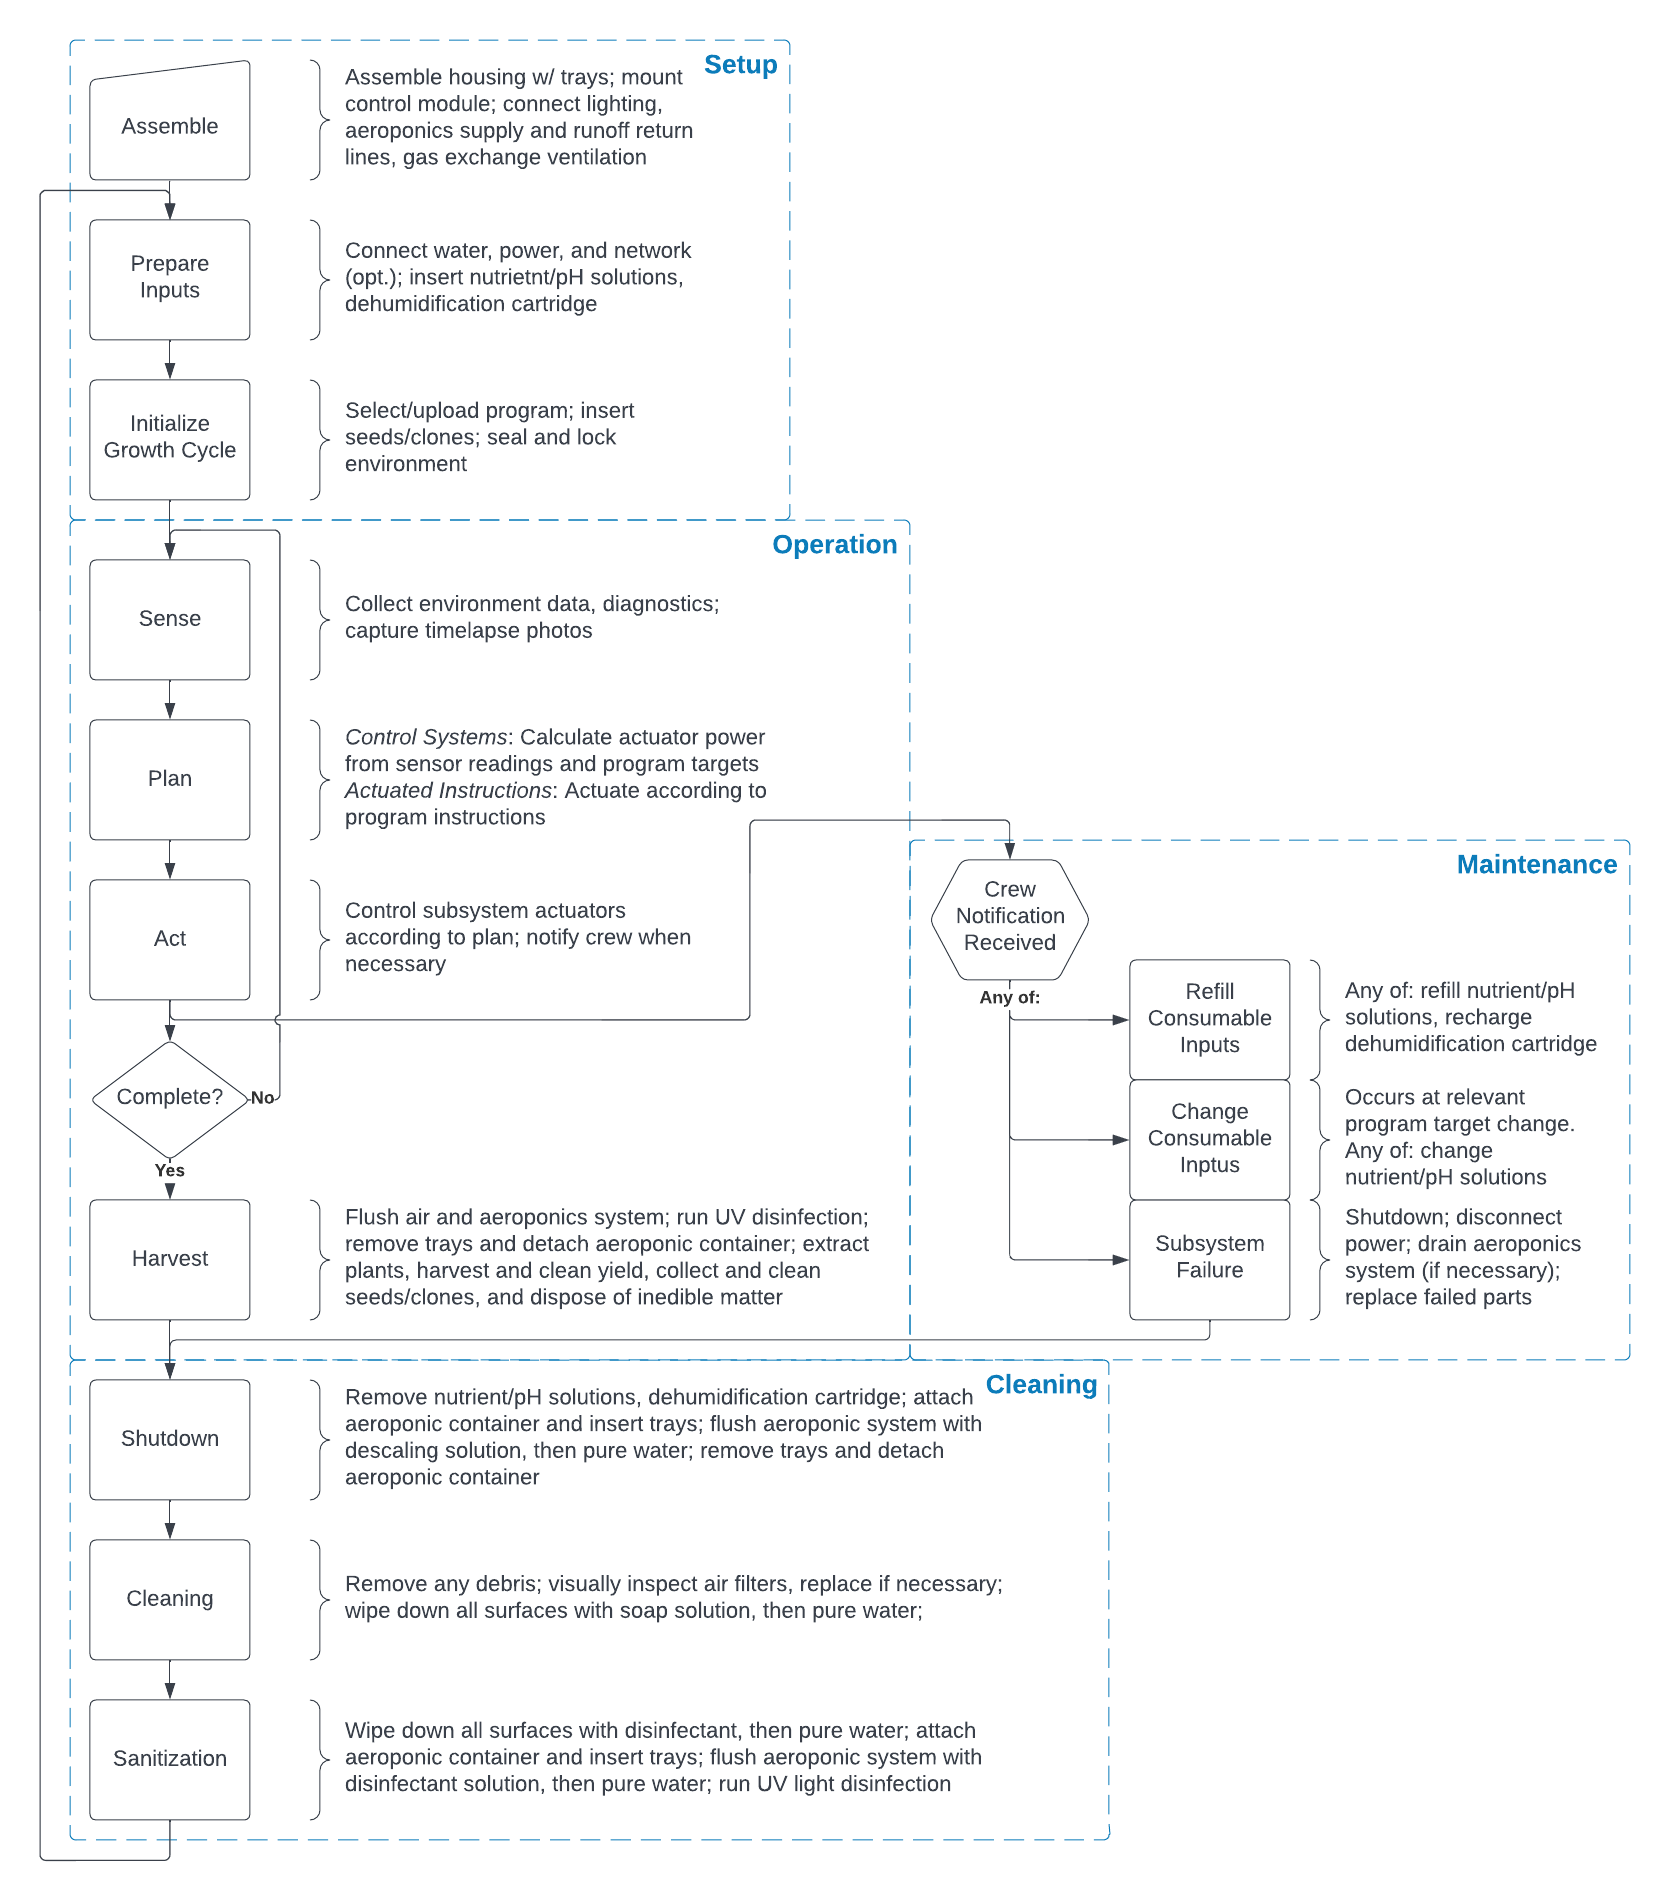
\includegraphics[width=0.9\textwidth]{../assets/figures/process.png}}
    \caption{Process diagram.}
    \label{fig:process}
\end{figure}

\clearpage

\subsubsection{Setup}
\label{sec:process_setup}

\textbf{Assembly}:
\begin{enumerate}
    \item Assemble housing, trays (see \ref{sec:housing});
    \item Mount control module, trays (see \ref{sec:housing});
    \item Connect subsystems to control module:
    \begin{itemize}
        \item \textit{Housing Solenoid Lock}: relay (see \ref{sec:housing})
        \item \textit{Aeroponics Supply \& Runoff Collection Lines}: quick-disconnect (see \ref{sec:aeroponics})
        \item \textit{Lighting Driver Board}: power, control signal (see \ref{sec:lighting})
    \end{itemize}
    \item Connect gas exchange exhaust to ventilation (see \ref{sec:gas});
\end{enumerate}

\textbf{Prepare Inputs}:
\begin{enumerate}
    \item Connect supply inputs:
    \begin{itemize}
        \item \textit{Power}: 120V 60Hz AC (see \ref{sec:automation});
        \item \textit{Network}: ethernet or wireless, optional (see \ref{sec:automation})
        \item \textit{Water}: reverse-osmosis, ambient (see \ref{sec:aeroponics})
    \end{itemize}
    \item Insert consumable inputs:
    \begin{itemize}
        \item \textit{Nutrient/pH Adjusment Solutions}: pouches (see \ref{sec:aeroponics})
        \item \textit{Dehumidification Cartridge}: recharged (see \ref{sec:dehumidification})
    \end{itemize}
\end{enumerate}

\textbf{Initialize Growth Cycle}:
\begin{enumerate}
    \item Select or upload program;
    \item Insert seeds/clones;
    \item Seal and lock environment;
    \item Start growth cycle;
\end{enumerate}

\textbf{Proceed to Operation} (see \ref{sec:process_operation}).

\subsubsection{Operation}
\label{sec:process_operation}

\textbf{Sense, Plan, Act} represent the three simultaneous automatic processes of the program's execution (see \ref{sec:automation}).

\textbf{Sense}:
Environment data, diagnostic information, and timelapse photos are captured and stored at regular intervals;

\textbf{Plan}:\\
\textit{Control Systems}: Actuator controls are calculated from sensor readings and program targets.\\
\textit{Actuated Instructions}: Actuator controls are derived from program instructions.

\textbf{Act}:
Subsystem actuators are controlled according to plan. Crew is notified to refill consumable inputs when low, change consumable inputs on program target change, and on any subsystem failure (see \ref{sec:process_maintenance}), as well as when to harvest and on End of Program (EoP).

\clearpage

\textbf{Harvest and/or EoP}:
\begin{enumerate}
    \item All air is exhausted (automatic, see \ref{sec:gas});
    \item Flush aeroponics system with pure water (automatic, see \ref{sec:aeroponics});
    \item Run UV disinfection (automatic, see \ref{sec:lighting});
    \item Unlock and open environment;
    \item Remove trays (see \ref{sec:housing}) and detach aeroponic container (see \ref{sec:aeroponics});
    \item \textbf{If EoP}: Extract plants;
    \item Harvest and clean yield;
    \item Collect, clean, and store seeds/clones;
    \item \textbf{If EoP}: Dispose of inedible matter;
\end{enumerate}

\textbf{If EoP, proceed to Cleaning} (see \ref{sec:process_cleaning})\textbf{. Otherwise, seal and lock environment and resume program.}

\subsubsection{Maintenance}
\label{sec:process_maintenance}

\textbf{Notification Handling}:
\begin{itemize}
    \item \textit{Refill Consumable Inputs}: includes refilling nutrient/pH adjustment solutions (see \ref{sec:aeroponics}), recharging the dehumidification cartridge (see \ref{sec:dehumidification})
    \item \textit{Change Consumable Inputs}: includes changing nutrient/pH adjustment solutions (see \ref{sec:aeroponics})
    \item \textit{Subsystem Failure}: all operation stopped, proceed to \textit{Shutdown} (see \ref{sec:process_cleaning}), disconnect power (see \ref{sec:automation}), then drain aeroponics system if necessary (see \ref{sec:aeroponics}) and replace failed components
\end{itemize}

\subsubsection{Cleaning}
\label{sec:process_cleaning}

\textbf{Shutdown}:
\begin{enumerate}
    \item Remove nutrient/pH solutions (see \ref{sec:aeroponics}), dehumidification cartridge (see \ref{sec:dehumidification});
    \item Attach aeroponic container (see \ref{sec:aeroponics}) and insert trays (see \ref{sec:housing});
    \item Flush aeroponic system with descaling solution (see \ref{sec:aeroponics});
    \item Flush aeroponic system with pure water (see \ref{sec:aeroponics});
    \item Remove trays (see \ref{sec:housing}) and detach aeroponic container (see \ref{sec:aeroponics});
\end{enumerate}

\textbf{Cleaning}:
\begin{enumerate}
    \item Visually inspect all surfaces for debris (remove) and components for damage (replace);
    \item Visually inspect all air filters (see \ref{sec:dehumidification}, \ref{sec:gas}), replace if necessary;
    \item Wipe down all surfaces with soap solution;
    \item Wipe down all surfaces with pure water;
\end{enumerate}

\textbf{Sanitization}:
\begin{enumerate}
    \item Wipe down all surfaces with disinfectant solution;
    \item Wipe down all surfaces with pure water;
    \item Dry all surfaces;
    \item Attach aeroponic container (see \ref{sec:aeroponics}) and insert trays (see \ref{sec:housing});
    \item Flush aeroponic system with disinfectant solution (see \ref{sec:aeroponics});
    \item Flush aeroponic system with pure water (see \ref{sec:aeroponics});
    \item Seal and lock environment;
    \item Run UV sanitization (\ref{sec:lighting});
\end{enumerate}

\textbf{Proceed to Prepare Inputs} (see \ref{sec:process_setup}).

\clearpage

\section{System-Level Report}
% To be extracted as a separate PDF and submitted as 1.3

\subsection{Automation}
\label{sec:automation}

\textbf{Purpose}: Performing growth-, maintenance-, and data-related tasks autonomously on the basis of both schedule and necessity to reduce crew maintenance time, improve consistency of products, and eliminate safety risks. Maintains the homogeneity of the internal environment with increased accuracy and precision over crew interference, while enabling simultaneous control over all parameters.

\textbf{Function}:
\begin{itemize}
    \item \textbf{Inputs}: Environment data stream (sensor readings), growth program
    \item \textbf{Outputs}: Actuator control signals, crew/cloud messaging, environment data (stored), timelapse photo set
\end{itemize}

\textbf{Method}:
\begin{enumerate}
    \item \textit{Setup}:
    \begin{enumerate}
        \item Power is connected and system is booted;
        \item Program is selected by user;
    \end{enumerate}
    \item \textit{Testing}:
    \begin{itemize}
        \item Power-on Self-Test (POST) passes (i.e. all hardware is online and communicating as expected).
        \item Systems enact program as intended (i.e. control systems respond properly).
    \end{itemize}
    \item \textit{Process}:
    \begin{enumerate}
        \item Checks operating preconditions (self POST and per-subsystem);
        \item \textbf{Environment Control Loop} (matches \textit{Sense-Plan-Act} model of robotics): %TODO cite the model
        \begin{enumerate}
            \item \textit{Sense}: Receives and stores data about current environment state;
            \item \textit{Plan}: Compares current state to "desired"/program state, develops a "plan"/actuator control to reach desired state;
            \item \textit{Act}: Controls subsystem operations in order to enact the plan;
        \end{enumerate}
        \item Notifies user on maintenance requirement (i.e. non-automated input/output management, refills, repairs, etc.), end-of-program (EoP), and diagnostic info;
    \end{enumerate}
    \item \textit{Shutdown} (either manual or EoP):
    \begin{enumerate}
        \item Stop all subsystem operations;
        \item Power down;
    \end{enumerate}
\end{enumerate}

\clearpage

\textbf{Features}:

A dual-computer system was chosen to allow for discrete management of high-level functionality (camera capture, internet/cloud functionality, local storage, complex calculations, etc.) and low-level functionality (hardware-level communications, actuator control and GPIO) in a master/slave topology with a constant two-way stream of shared data.

\begin{itemize}
    \item \textit{Computer (Master)} \cite{raspberrypi}: Manages data collection, batch storage, analysis, and transmission/receiving, as well as planning/calculations for actuator control. Includes internal clock (for program, notification), network connection (for data transmission, notification), photo capture, and non-volatile storage (for data/photos). Sends instructions derived from the program to the microcontroller.
    \item \textit{Microcontroller (Slave)} \cite{arduino}: Manages detailed sensor/actuator states and communications (on/off, sensor readings, actuator control). Streams collected sensor readings to the computer.
    \item \textit{Program}: Set of actuated instructions (e.g. lights on) and control targets (e.g. hold air temperature at 22°C) to enact at specific points in the growth cycle, as well as config data;
    \item \textit{Camera Capture \& Plant Performance Metric (PPM) Extraction}: Top-down and side-view cameras \cite{camera}, captured under standard lighting at regular intervals throughout the course of the growth cycle. For live feed transmission to users (local and remote), as well as PPM extraction via computer vision and machine learning for yield and diagnostic analysis. Potentially relevant PPMs include (but are not limited to):
    \begin{itemize}
        \item Leaf health indicators (i.e. leaf tip burn, leaf curl, chlorosis);
        \item Leaf count, size distribution;
        \item Leaf density;
        \item Canopy dimensions/surface area;
        \item Plant height;
        \item Fruit/harvest body size, ripeness;
    \end{itemize}
    \item \textit{Environment Data}: Record the environment's current state. Covers each \textit{control system} environment parameter (e.g. included in a feedback loop). Control system environment parameters include:
    \begin{itemize}
        \item Leaf-zone temperature (see \ref{sec:airthermoregulation});
        \item Leaf-zone humidity (see \ref{sec:humidityregulation});
        \item Root-zone temperature (see \ref{sec:aeroponics});
        \item Gas concentrations (see \ref{sec:gas});
    \end{itemize}
    \item \textit{Actuator Control}: Induces change in environment parameters. Covers both \textit{control system} and \textit{actuated instruction} environment parameters. Actuated instruction environment parameters include:
    \begin{itemize}
        \item Lighting (see \ref{sec:lighting});
        \item Water delivery (see \ref{sec:aeroponics});
        \item Plant nutrient delivery (see \ref{sec:aeroponics});
        \item Water pH (see \ref{sec:aeroponics});
        \item Air circulation rate (see \ref{sec:airthermoregulation});
    \end{itemize}
    \item \textit{Diagnostic Systems}: Include informative sensors tracking system input availability, subsystem diagnostics, etc. as well as notification triggers.
\end{itemize}

\clearpage

\textbf{Figures}

\begin{figure}[h!]
    \centering
    \frame{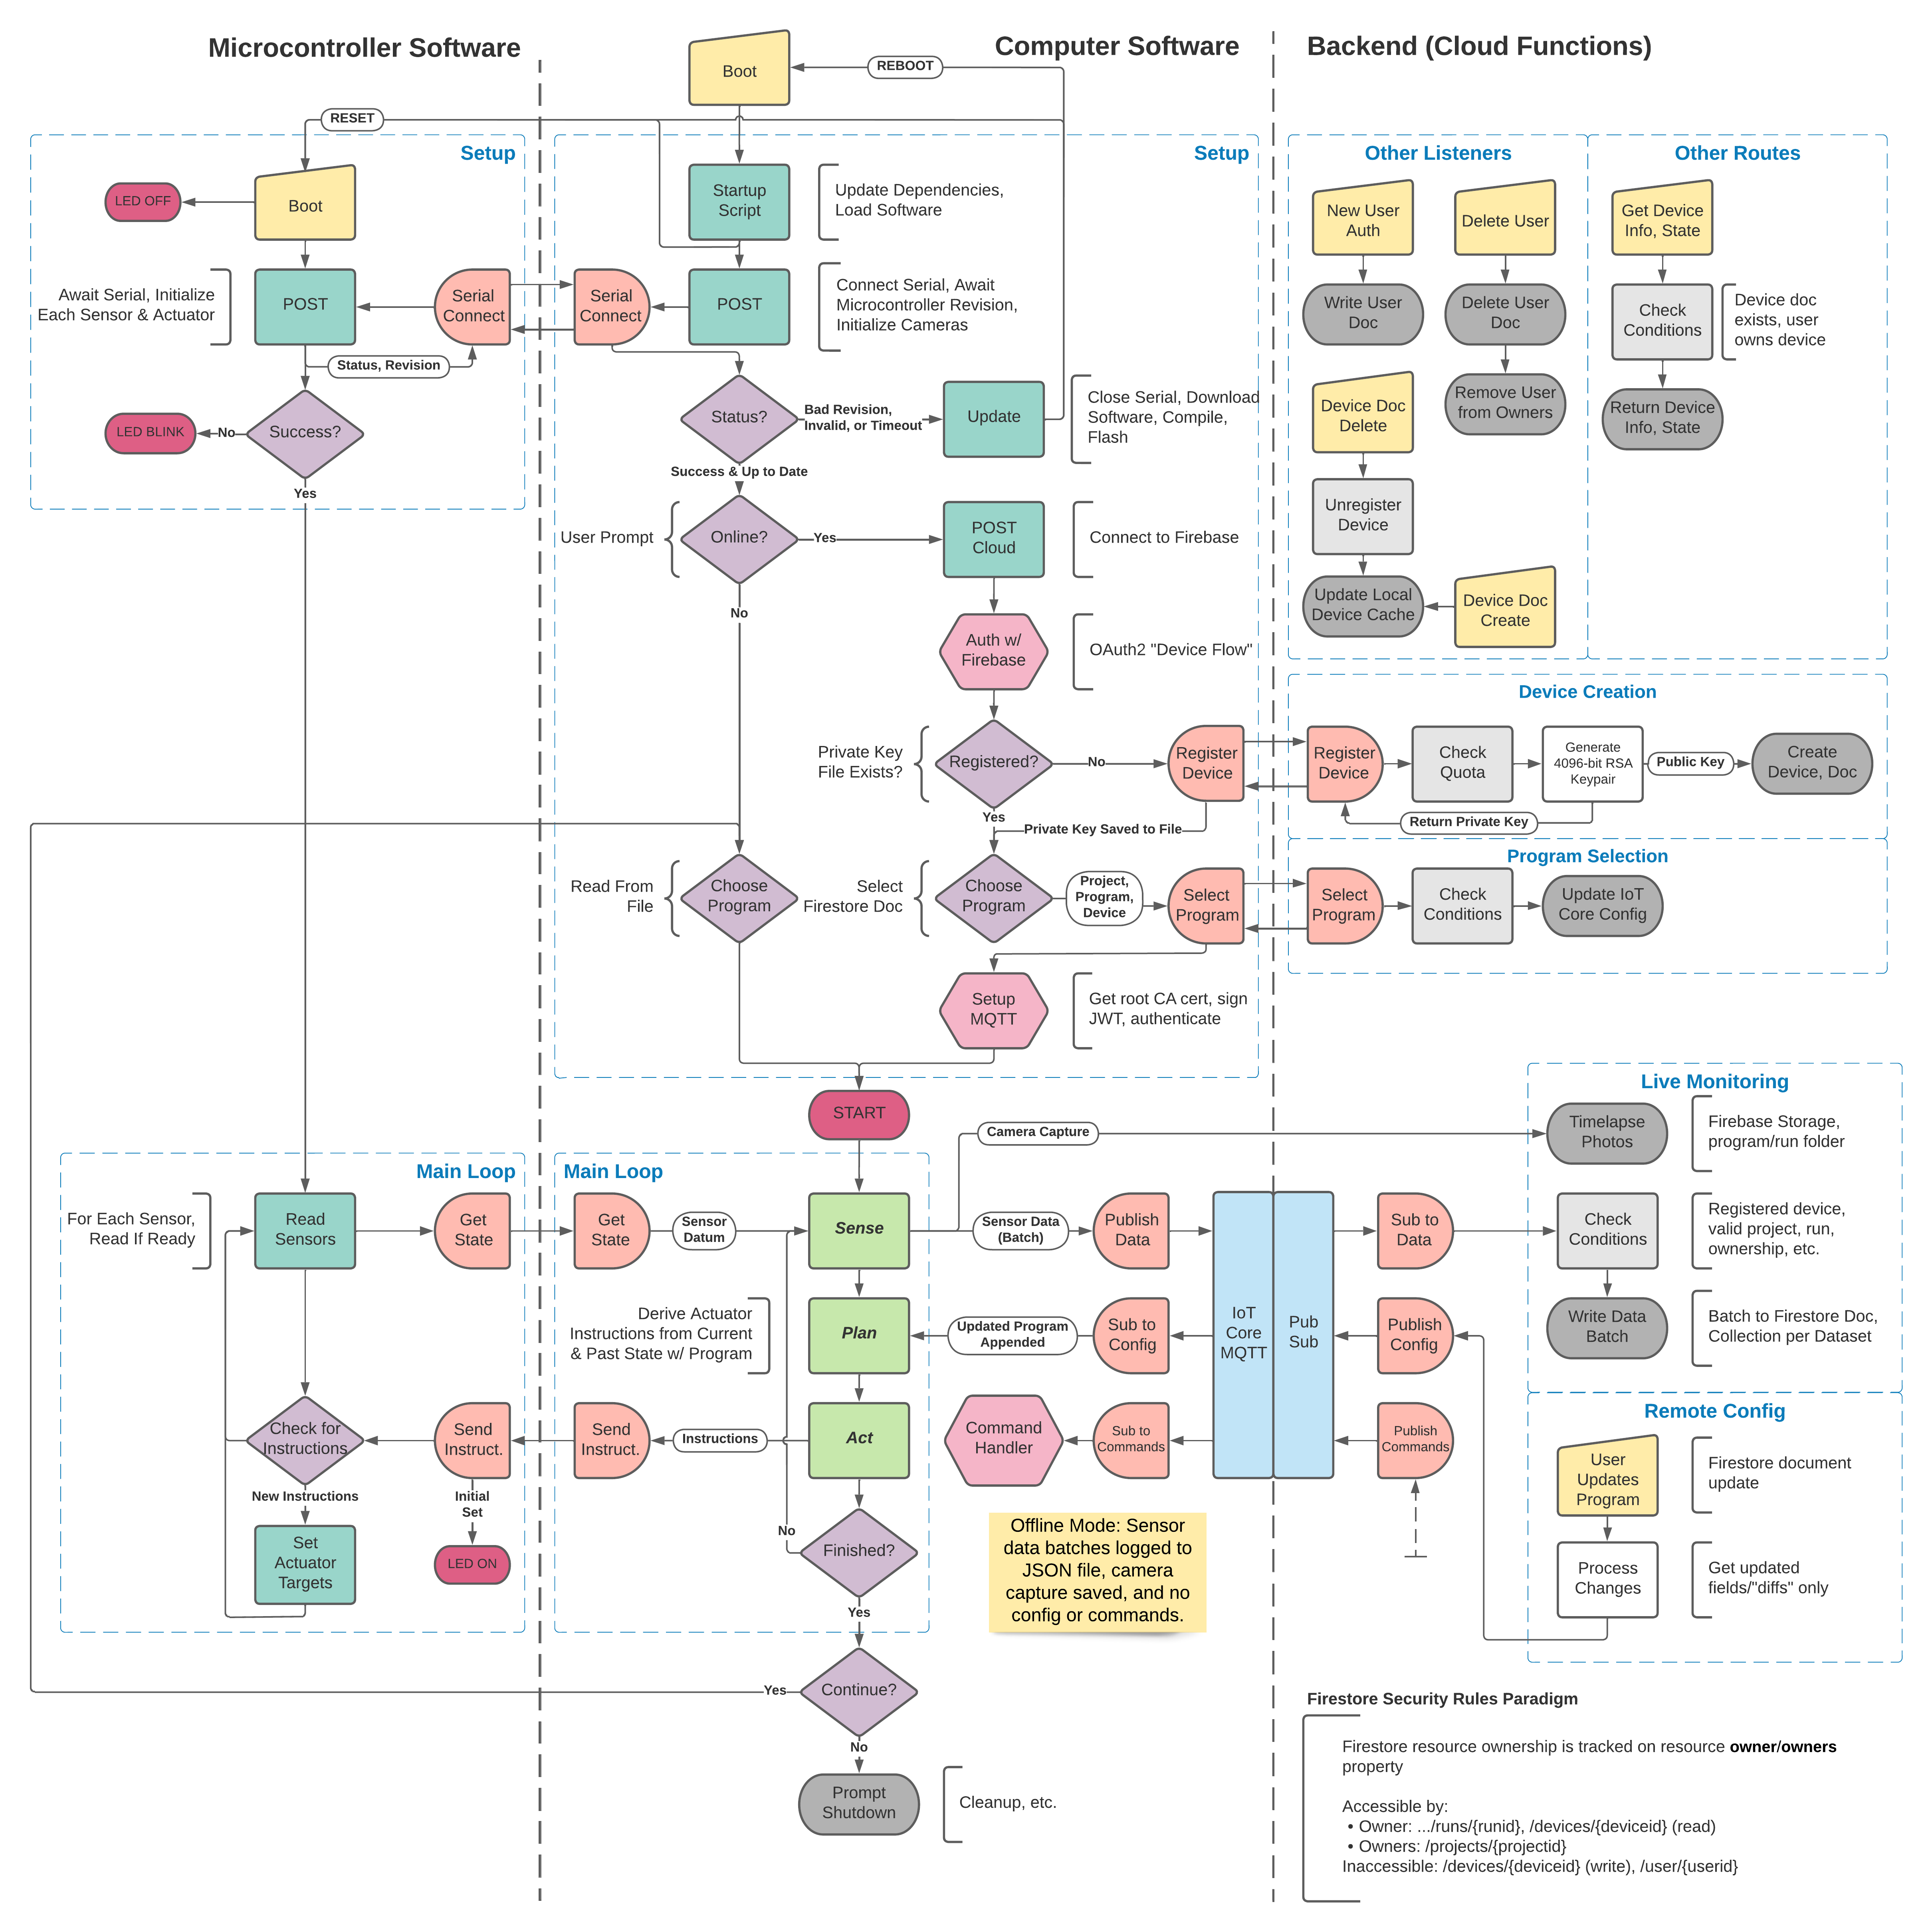
\includegraphics[width=\textwidth]{../assets/figures/automation_software.png}}
    \caption{Software control flow diagram.}
    \label{fig:automation_software}
\end{figure}

\begin{figure}[h!]
    \centering
    \frame{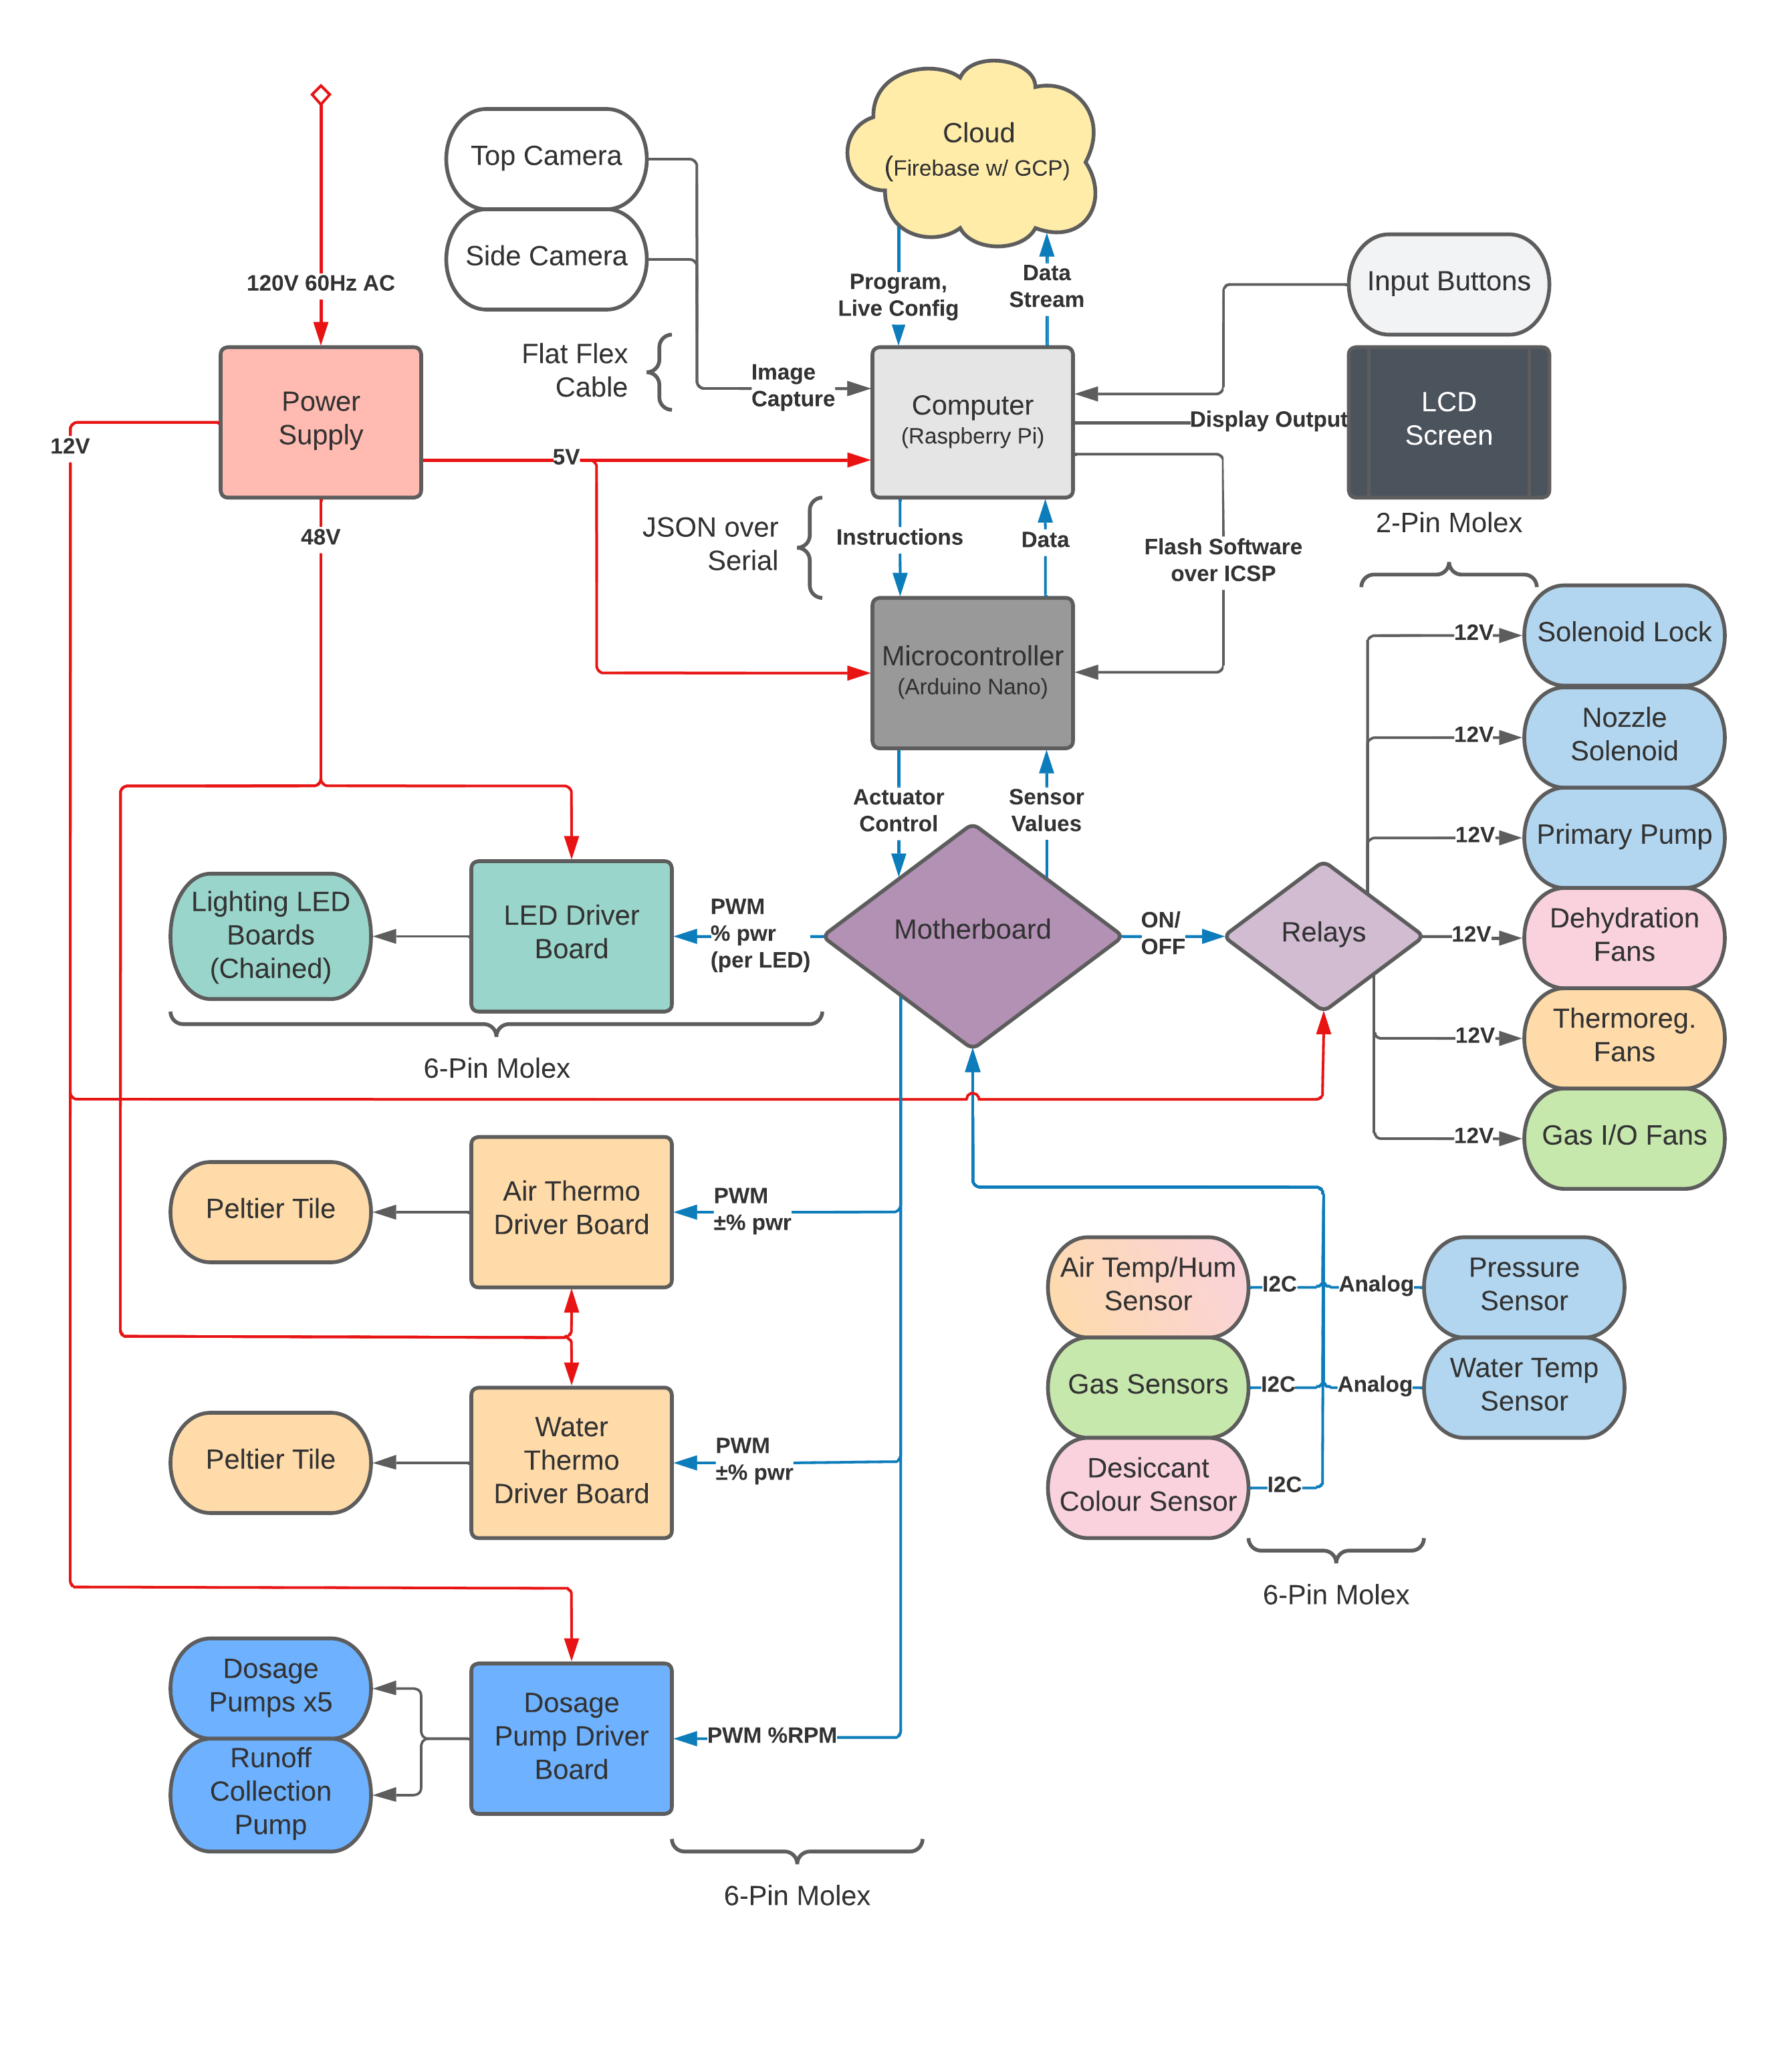
\includegraphics[width=\textwidth]{../assets/figures/automation_wiring.png}}
    \caption{System wiring diagram.}
    \label{fig:automation_wiring}
\end{figure}

\clearpage

\subsection{Housing}

\begin{figure}[h!]
  \centering
  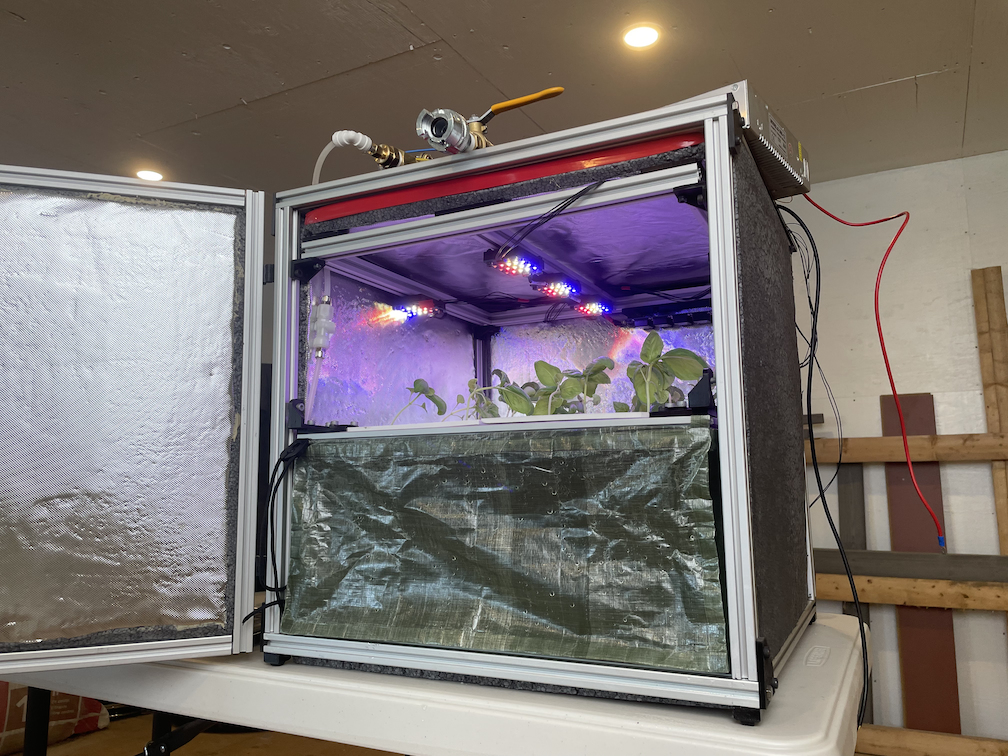
\includegraphics[width=\textwidth]{../assets/photos/prototype_housing.png}
  \hfill
  \caption{Housing prototype. Note lighting and grow trays, as well as reflective sheet-laminated foam insulation panels.}
  \label{fig:prototype_housing}
\end{figure}

The prototype performs all functions as designed.

\clearpage

\subsection{Aeroponics}
\label{sec:aeroponics}

\textbf{Purpose}: Delivers plant nutrients and pH- and temperature-controlled water to the roots via a fine mist.

\textbf{Function}:
\begin{itemize}
    \item \textbf{Inputs}: Reverse osmosis water\footnote{RO water has no dissolved nutrients and a neutral pH of 7.0. This enables easier and more reliable calculations. In addition, it has no particulate or minerals, minimizing the chances of nozzle clog.} under positive pressure, concentrated pH up \& down solutions and nutrient solutions, nozzle delivery on/off control (\ref{sec:automation}), pH and nutrient solution ratios as control signals (dosing pump speeds; \ref{sec:automation}), water thermoregulation control signal (\ref{sec:automation})
    \item \textbf{Outputs}: pH- and nutrient-controlled water mist (50 micron mean droplet diameter)
\end{itemize}

\textbf{Method}:
\begin{enumerate}
    \item \textit{Setup}:
    \begin{enumerate}
        \item Hook up water, solution, and signal inputs;
        \item Connect the quick-disconnect fitting;
        \item Calibrate pressure, temperature sensors to atmospheric;
        \item Enable water input to prime system (if known pressure/temperature, calibrate sensors);
        \item Mount container, connect runoff collection line to recycling port;
    \end{enumerate}
    \item \textit{Testing}:
    \begin{itemize}
        \item Temperature, pressure sensors communicate as expected;
        \item No leaks at any connections under a) source pressure, b) fully pressurized;
        \item Pump actuates and auto-shuts off as expected, and is able to deliver the required pressure;
        \item All components, tubing, and connectors/fittings withstand full pressurization;
        \item Solenoid is normally closed, withstands full pressurization, and opens when power is applied;
        \item Quick-disconnect operates as intended at full pressurization without leaks;
        \item Nozzles produce even-distribution full-cone mist;
        \item Manual and actuated valves operate as intended;
        \item Runoff container is sealed, and runoff collection operates as intended;
    \end{itemize}
    \item \textit{Process}:
    \begin{enumerate}
        \item Water is pressurized to constant 80psi;
        \item Heat is added to or removed from the water;
        \item Temperature and pressure of the water is read (feedback);
        \item Nutrient and pH solutions are mixed in-line at an adjustable ratio\footnote{I.e. add X mL of nutrient solution Y per mL water to achieve Z ppm, or add A mL of pH down solution per mL water to achieve a pH of B.};
        \item Flow to nozzle is controlled (on/off);
        \item Nozzle turns pressurized water into mist;
        \item Runoff is contained by a water-tight container, and collected for recycling;
    \end{enumerate}
    \clearpage
    \item \textit{Shutdown}:
    \begin{enumerate}
        \item Power down the pump and thermoregulation unit;
        \item Close the nutrient and pH solution valves;
        \item Close the source shutoff valve;
        \item Open the drain valve, and allow the system to depressurize completely;
        \item Re-open the source shutoff valve and flush the system with fresh water;
        \item Power down the solenoid;
        \item Collect all remaining runoff;
        \item Disconnect the quick-disconnect fitting;
        \item Disconnect the inputs;
    \end{enumerate}
\end{enumerate}

\textbf{Features}:
\begin{itemize}
    \item \textit{Water Source}: Input for ambient reverse-osmosis water.
    \item \textit{Manual Source Shutoff Valve}: Ball valve.
    \item \textit{Diaphragm Pump}: Self-priming, auto-shutoff at 80psi. Power is controlled by a relay.
    \item \textit{Inline Thermoelectric Water Heater/Cooler Block}: Aluminum water block heat pump. See Section \ref{sec:airthermoregulation}.
    \item \textit{PID Control Loop}: A propotional-integral-derivative control loop enables increased accuracy (see equation \ref{eqn:pid}, \ref{sec:airthermoregulation}).
    \item \textit{Solution Injection Manifold}: A manifold of parallel inline injectors, allowing for on-demand adjustment of mixing ratios for nutrient and pH solutions. Comprises:
    \begin{itemize}
        \item \textit{Manifold}: Splits the water line into a set of parallel branches with inline tees to enable solution injection.
        \item \textit{Dosing Pumps}: Stepper-motor driven custom peristaltic pumps deliver solutions at a controlled rate/ratio (one per solution). Toleranced to prevent backflow at pressure. % TODO more details (tubing type, washers, bearings, etc.) w/ part numbers
        \item \textit{Nutrient Solutions}: Aqueous. Highly concentrated. Selectable as part of the program (\ref{sec:automation})\footnote{Many different solutions can be combined (according to solubility laws, pH requirements, etc.).}, and may include any of:
        \begin{itemize}
            \item Bioavailable nonmetals (ammonia, ammonium, nitrates, nitrites, phosphates, sulfates, etc.)
            \item Bioavailable metals (potassium, etc.)
            \item Minerals (magnesium, calcium)
            \item Other trace elements
            \item Custom solutions (i.e. fungicides/algicides, descaling solutions)
        \end{itemize} 
        \item \textit{pH Adjustment Solutions}\footnote{\textit{NOTE:} Ionic composition of pH solutions should be considered in the understanding of the nutrient composition (i.e. phosphic acid results in phosphate ions in spray)}: Aqueous. Highly concentrated. One for pH up (>8), one for pH down (<6).
        \item \textit{Solution Storage Containers}: Opaque, insulated, chemical-safe, refillable cartridges. Prevent degradation of solution compounds over time via light or heat.
        \begin{itemize}
            \item \textit{Fill Level Sensors}: Depth sensors measure fill level of container. Notifies user to refill.
        \end{itemize}
    \end{itemize}
    \item \textit{Water Temperature Sensor}: Tee-fitted. Informs a \textbf{PID control loop}. See Section \ref{sec:airthermoregulation}.
    \item \textit{Accumulator Tank}: Uses an air bladder to maintain and stabilize pressure.
    \item \textit{Pressure Sensor}: Allows for shutoff of pump in case of emergency.
    \item \textit{Drain Valve}: Tee-fitted ball valve. Allows the system to be depressurized and drained.
    \item \textit{Solenoid Valve}: Controls delivery to the nozzles to enable on-demand misting.
    \item \textit{Grow Tray Quick-Disconnect}: Connectors between aeroponics supply and nozzles that allow for quick disconnection with auto-shutoff so the trays may be removed.
    \item \textit{Nozzle}: Mounted to grow tray, pointed at plant roots. 80psi water through a 0.4-0.6mm orifice produces 5-50 micron water droplets, optimal for plant growth. This method is 98\% more water-efficient than traditional farming.%TODO: Sources??
    \item \textit{Root-Zone Container}: Watertight container that encapsulates the entire root zone. Made of a woven waterproof composite fabric (CT5K.18 mylar with Dyneema, 1.43oz/yd${}^2$ or 33.89g/m${}^2$), chosen for high strength-to-weight ratio (15x that of steel) and natural no-coating food-safe waterproof quality \cite{dyneema}. Mounted and \textbf{sealed} to the grow tray with a drawstring for easy root zone access. Provides water supply and runoff collection ports.
\end{itemize}

\textbf{Figures}

\begin{figure}[h!]
    \centering
    \frame{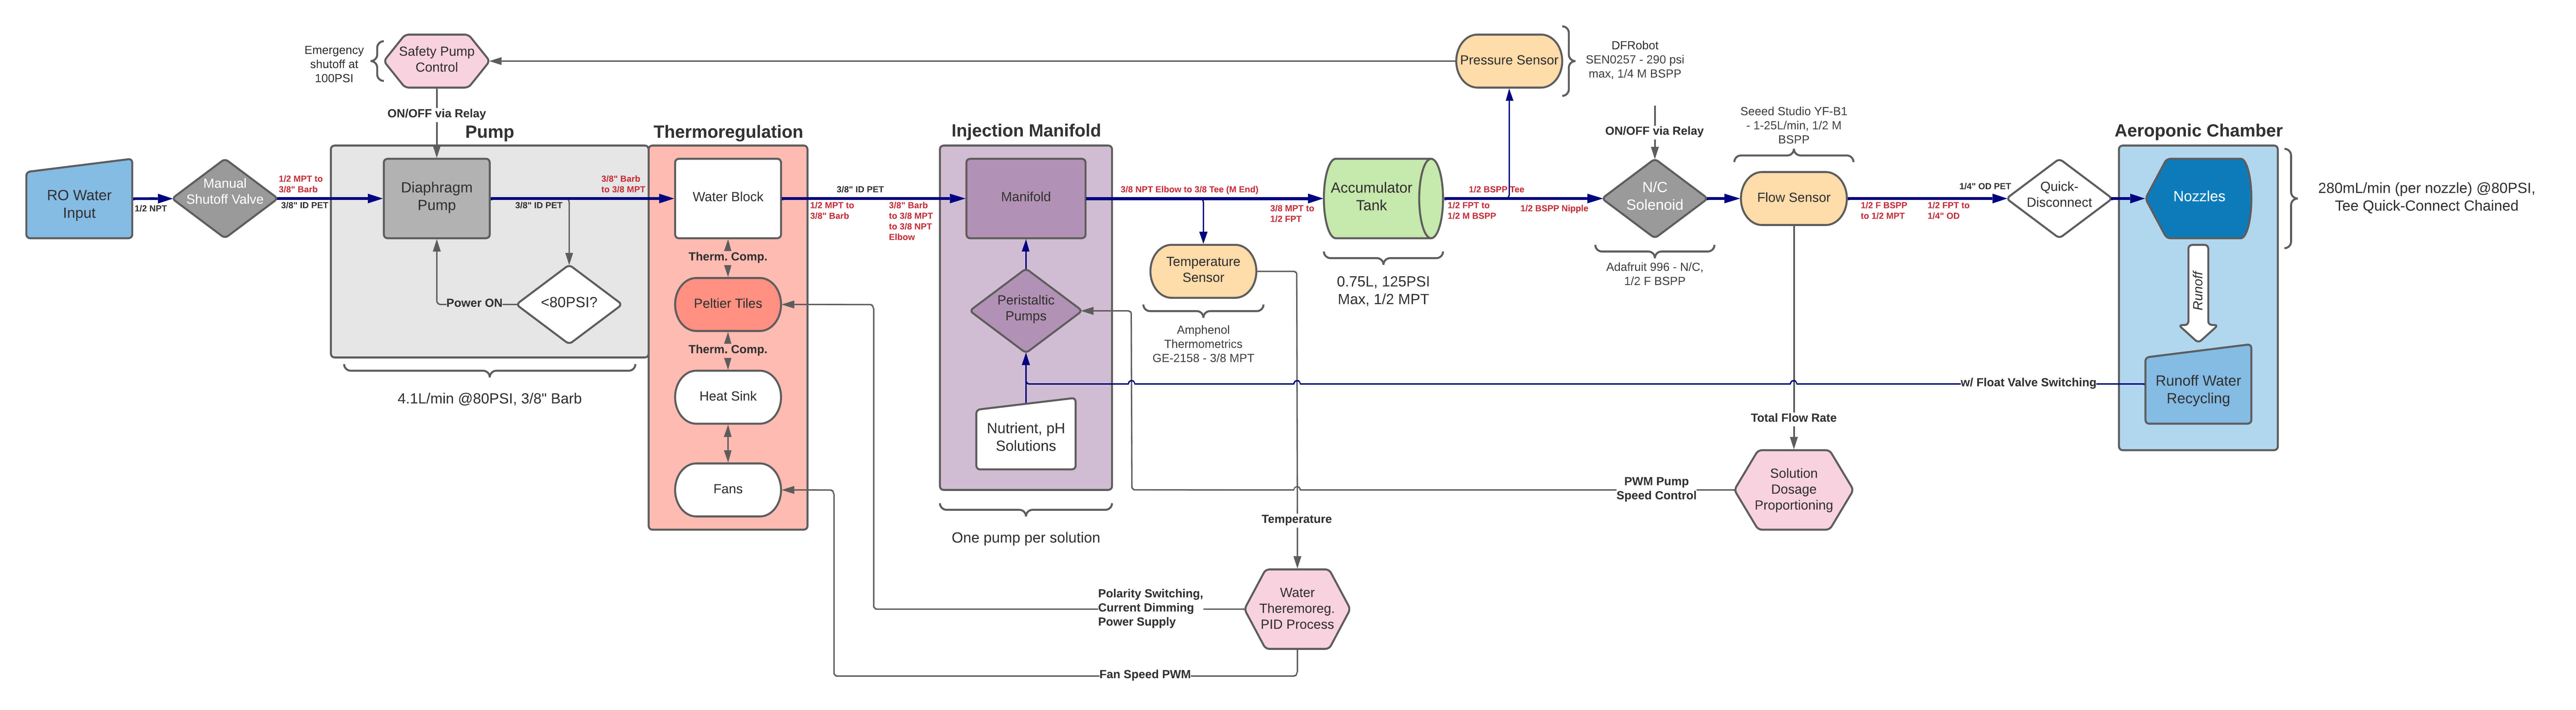
\includegraphics[width=\textwidth]{../assets/figures/aeroponics_plumbing.png}}
    \caption{Aeroponics plumbing diagram.}
    \label{fig:aeroponics_plumbing}
\end{figure}

\begin{figure}[h!]
    \centering
    \frame{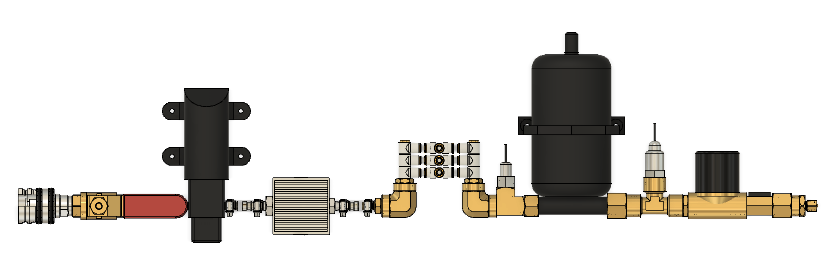
\includegraphics[width=\textwidth]{../assets/figures/aeroponics_supply.png}}
    \caption{Aeroponics supply system.}
    \label{fig:aeroponics_supply}
\end{figure}

% TODO Pump model figure

\clearpage

\clearpage

\subsection{Leaf-Zone Thermoregulation}
\label{sec:airthermoregulation}

\textbf{Purpose}: Maintaining desired leaf-zone air temperature and circulating air.

\textbf{Function}:
\begin{itemize}
    \item \textbf{Inputs}: Power, air temperature control signal (\ref{sec:automation}), air circulation control signal (\ref{sec:automation})
    \item \textbf{Outputs}: Heat to/from environment, by-product heat from/to surroundings, internal air circulation, internal air temperature sensor readings (\ref{sec:automation})
\end{itemize}

\textbf{Method}:
\begin{enumerate}
    \item \textit{Testing}:
    \begin{itemize}
        \item Heat pump direction and magnitude respond to control signal as expected;
        \item Fans operate as expected;
        \item Heat pump power exceeds maximum heat loss (temperature extremes)\footnote{i.e. if X Watts leave the system at MAX$\degree$C internal, and Y Watts enter the system at MIN$\degree$C internal, the heat pump must transfer >X, >Y Watts.};
        \item Heat pump power exceeds that required to reach temperature extremes in under 120 seconds given the system's heat capacity;
    \end{itemize}
    \item \textit{Process}:
    \begin{enumerate}
        \item Air is circulated throughout the environment;
        \item Temperature is measured, sent to automation system (\ref{sec:automation});
        \item Control module controls heat pump speed and direction (heating vs. cooling environment, \ref{sec:automation});
    \end{enumerate}
\end{enumerate}

\textbf{Calculations}:

Assuming an atmospheric pressure $P$ of 101.325kPa, a surroundings temperature range $T_{surr}$ of 22$\degree$C, a system target temperature range $[T_{sys-min}$, $T_{sys-max}]$ of 10-35$\degree$C, a molar mass of dry air $M$ of 28.97 $\frac g{mol}$, a specific heat capacity of dry air $c_p$ of $1.006 \frac{J}{g*\text{K}}$\footnote{Water vapour has a maximum concentration of 30g/kg at 30$\degree$C, or 3\%, which is negligible for mass and heat capacity calculations.}, a 4U Class 2 expanded configuration (2x2 units, 16 faces; see \ref{sec:housing}), and a face insulation RSI per mm of $0.0328\text{m}^2~  \degree \text{C}~\text{W}^{-1}~\text{mm}^{-1}$ (see \ref{sec:housing}):\\
\vspace{.05cm}
\begin{gather}
    \label{eqn:heatloss}
    Q_{loss}=\frac{(T_{surr}-T_{sys-max}) * A}{\text{RSI per mm} * \ell}=\frac{(22\degree \text{C}-35\degree \text{C}) * (16 \text{ faces} * 0.5\text{m} * 0.5\text{m})}{0.0328 \text{m}^2~  \degree \text{C}~\text{W}^{-1}~\text{mm}^{-1} * 25.4 \text{mm}}=-62.42 W\\
    \label{eqn:heatgain}
    Q_{gain}=\frac{(T_{surr}-T_{sys-min}) * A}{\text{RSI per mm} * \ell}=\frac{(22\degree \text{C}-10\degree \text{C}) * (16 \text{ faces} * 0.5\text{m} * 0.5\text{m})}{0.0328 \text{m}^2~  \degree \text{C}~\text{W}^{-1}~\text{mm}^{-1} * 25.4 \text{mm}}=57.61 W\\
    \label{eqn:airmass}
    m_{air}=\frac{P*V*M}{R*T_{avg}}=\frac{101325\text{Pa}*(0.5\text{m}*0.5\text{m}*0.5\text{m}*4\text{ units})*28.97\frac g{mol}}{8.314\frac{J}{\text{mol}*K}*300\text{K}}=588.4g\\
    \label{eqn:heating}
    Q_{heating}=\frac{m*c_p*(T_{surr}-T_{sys-max})}{t}=\frac{588.4g*1.006\frac{J}{g*\text{K}}*(22\degree \text{C}-35\degree \text{C})}{120\text{ sec}}=-64.13\text{W}\\
    \label{eqn:cooling}
    Q_{cooling}=\frac{m*c_p*(T_{surr}-T_{sys-min})}{t}=\frac{588.4g*1.006\frac{J}{g*\text{K}}*(22\degree \text{C}-10\degree \text{C})}{120\text{ sec}}=59.19\text{W}
\end{gather}

\clearpage

$\therefore$ A thermoelectric system able to transfer at least \textbf{70W} (such as \cite{peltier}, which transfers up to 85W) will supply enough power to heat/cool the system from ambient to extremes in 120 seconds and maintain temperature.

\begin{gather}
    \label{eqn:thermalresistance-hot}
    R_{\theta~Peltier-Surr}=R_{\theta~Peltier-Sink}+R_{\theta~Sink-Air}\le\frac{T_{h~max} - T_{surr}}{Q_{max}}=\frac{50\degree C - 22\degree C}{85W}=0.329\degree \text{C W}^{-1}\\
    \label{eqn:thermalresistance-cold}
    R_{\theta~Peltier-Sys}=R_{\theta~Peltier-Sink}+R_{\theta~Sink-Air}
\end{gather}

\textbf{Features}:
\begin{itemize}
    \item \textit{Circulation Fans}: Located in growth environment to circulate air for even temperature distribution, rapid system flushing, and automatic pollination.
    \item \textit{Temperature Sensors}: Multiple temperature and humidity sensors \cite{sht31} on small daughterboards frame-mounted throughout the growth environment to measure air temperature ($\degree$C). Informs the \textbf{PID control loop}.
    \item \textit{Heat Pump}: Pumps heat in or out of the growth environment. Is comprised of:
    \begin{itemize}
        \item \textit{Peltier Device}: 85W bidirectional solid-state \textbf{thermoelectric device} (aka Peltier tile) \cite{peltier} pumps heat from one face to the other. Better space efficiency, less complexity (no liquids, pressurized fluids, etc.), and more precise than other methods.
        \item \textit{Thermoelectric Driver Board}: Controls \textit{magnitude} and \textit{direction} of heat transfer via a \textbf{dimmable voltage source} (low-pass-filtered PWM to a voltage buffer and amplifier w/ feedback) and \textbf{relay H-bridge}, respectively. See Figures \ref{fig:peltierdriver} and \ref{fig:thermoregulation_driver}.
        \item \textit{Heat Sinks}: Aluminum blocks with fins hold and exchange heat between air and Peltier devices. One set on each side of the Peltier (inside and outside environment) builds "heat pump". Mating face coated with thermal compound for better transfer.
        \item \textit{Heat Sink Fans}: Located on both sets of heat sinks for better heat dissipation.
    \end{itemize}
    \item \textit{PID Control Loop}: A propotional-integral-derivative control loop enables increased accuracy (see equation \ref{eqn:pid}). Temperature sensors inform the loop, "error" is calculated (current vs desired temperature, see $E(t)$ \ref{eqn:piderror}), and this informs the magnitude and direction of heat pump control ($u(t)$). Requires tuning of parameters ($K_p, K_i, K_d$; automatic). Built into the automation system (see \ref{sec:automation});
\end{itemize}

\begin{gather}
    \label{eqn:piderror}
    E(t)=T_{target}(t)-T_{measured}(t)\\
    \label{eqn:pid}
    u(t)=K_pE(t)+K_i\int_0^{t}E(t)dt+K_d\frac{dE(t)}{dt}
\end{gather}

\clearpage

\textbf{Figures}

\begin{figure}[h!]
  \centering
  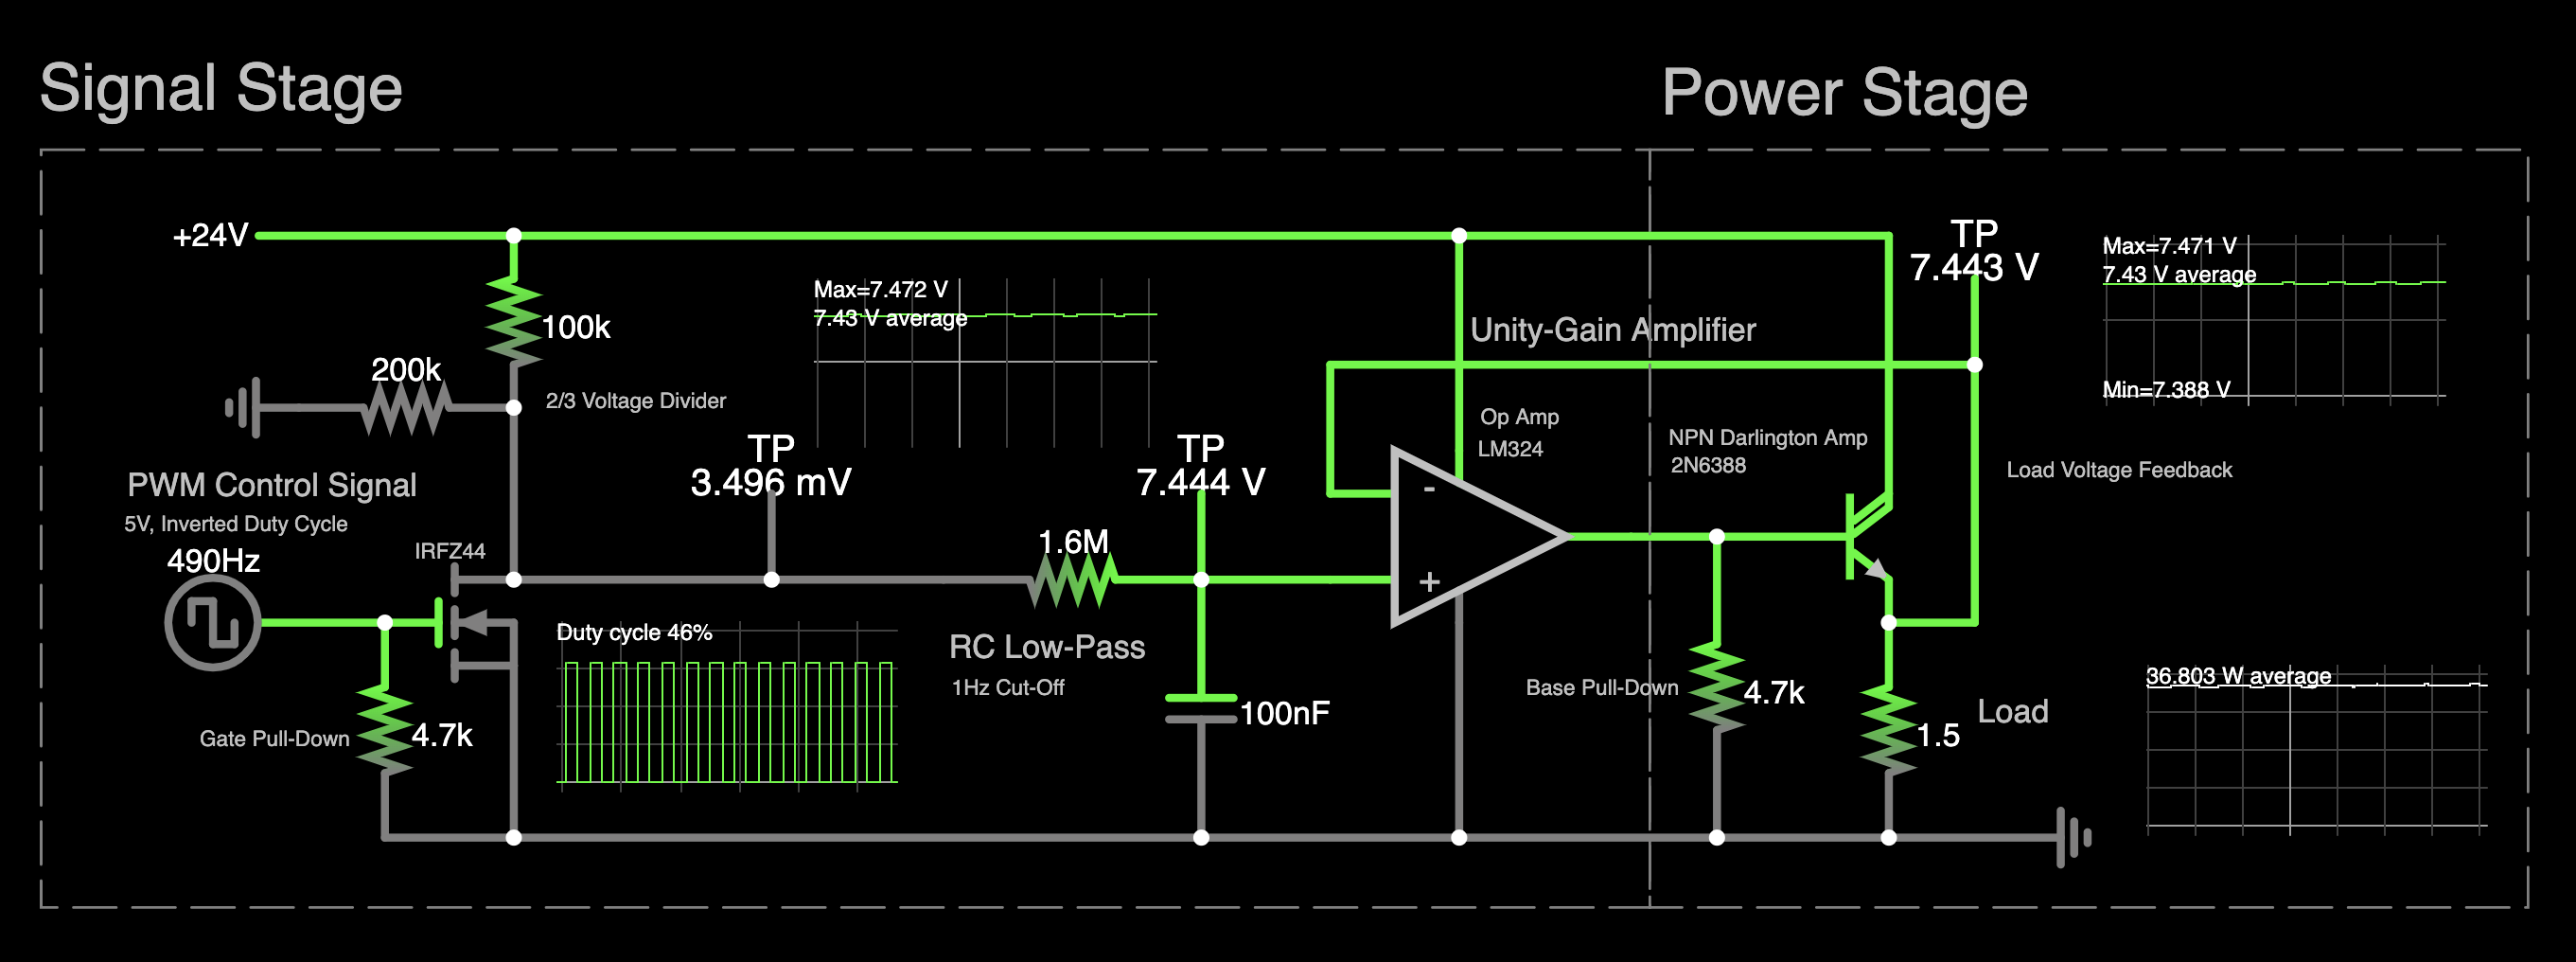
\includegraphics[width=\textwidth]{../assets/figures/airthermoregulation_simulation.png}
  \hfill
  \caption{Thermoelectric driver circuit simulation \cite{thermo-falstad}}
  \label{fig:peltierdriver}
\end{figure}

\begin{figure}[h!]
    \centering
    \begin{subfigure}{.49\textwidth}
        \centering
        \frame{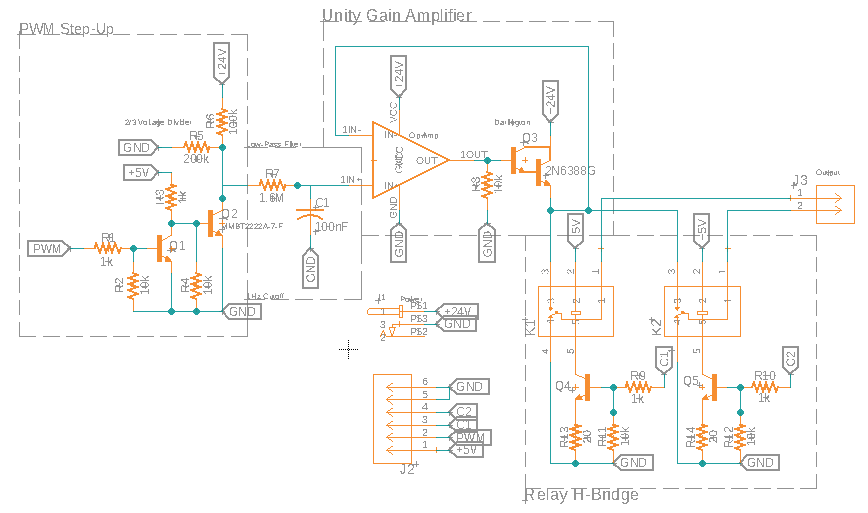
\includegraphics[width=\textwidth]{../assets/schematics/thermoregulation_driver_sch.png}}
        \caption{Schematic.}
        \label{fig:thermoregulation_driver_sch}
      \end{subfigure}
      \hspace{.02\textwidth}
      \begin{subfigure}{.43\textwidth}
        \centering
        \frame{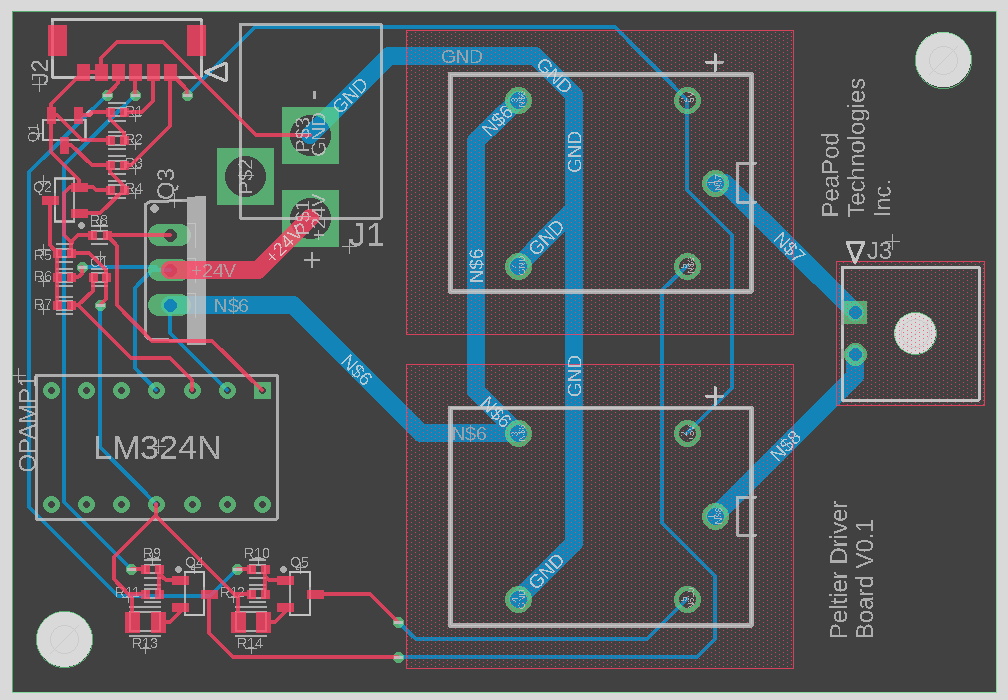
\includegraphics[width=\textwidth]{../assets/schematics/thermoregulation_driver_brd.png}}
        \caption{PCB layout.}
        \label{fig:thermoregulation_driver_brd}
      \end{subfigure}
      \caption{Thermoelectric driver board.}
      \label{fig:thermoregulation_driver}
\end{figure}

\clearpage

\clearpage

\subsection{Leaf-Zone Humidity Regulation}
\label{sec:humidityregulation}

\textbf{Purpose}: Regulates the relative humidity of the leaf zone.

\textbf{Function}:
\begin{itemize}
    \item \textbf{Inputs}: Humidification on/off control signal (\ref{sec:automation}), dehumidification on/off control signal (\ref{sec:automation})
    \item \textbf{Outputs}: Humidification or dehumidification on-demand
\end{itemize}

\textbf{Method}:
\begin{enumerate}
    \item \textit{Process}:
    \begin{enumerate}
        \item When humidity is too low (outside dead-zone), humidification is activated;
        \item When humidity is too high (outside dead-zone), dehumidification is activated;
        \item When humidity is at target (within dead-zone), both systems are deactivated;
    \end{enumerate}
\end{enumerate}

\textbf{Features}:
\begin{itemize}
    \item \textit{Humidification System}: See Section \ref{sec:humidification}.
    \item \textit{Dehumidification System}: See Section \ref{sec:dehumidification}.
    \item \textit{Humidity Sensors}: Multiple temperature and humidity sensors \cite{sht31} on small daughterboards frame-mounted throughout the growth environment to measure air relative humidity (\%RH). Informs the \textbf{bang-bang control loop}.
    \item \textit{Bang-Bang Control Loop}: A bang-bang (on/off) control loop with a hysteresis dead-zone (see equation \ref{eqn:bangbang}). Humidity sensors inform the loop, "error" is calculated (current vs desired humidity), and this informs whether or not to activate either the humidification or dehumidification systems (or neither). Requires tuning of dead-zone (automatic). Built into the automation system (see \ref{sec:automation});
\end{itemize}

\begin{gather}
    \label{eqn:bangbang}
    u(t)=\begin{dcases}
        -1  &   x < -d \\
        0   &   -d \leq x \leq d \\
        1   &   x > d \\
    \end{dcases}
\end{gather}

\clearpage

\subsubsection{Humidification}
\label{sec:humidification}

\textbf{Purpose}: Actively \textit{increases} growth environment air humidity.

\textbf{Function}:
\begin{itemize}
    \item \textbf{Inputs}: Power, humidification on/off control signal (\ref{sec:automation}), RO water\footnote{RO water contains no minerals/particulate, and as such prevents the common problem of mesh clog/calcification.};
    \item \textbf{Outputs}: Dry water vapour (\ref{sec:automation});
\end{itemize}

\textbf{Method}:
\begin{enumerate}
    \item \textit{Setup}:
    \begin{enumerate}
        \item Connect humidification control signal to control module;
        \item Connect RO water line to water tank;
    \end{enumerate}
    \item \textit{Testing}:
    \begin{itemize}
        \item Humidification unit responds to control signal as expected;
        \item Humidity sensor reads as expected;
        \item Tank does not leak;
    \end{itemize}
    \item \textit{Process}:
    \begin{enumerate}
        \item Water is delivered to a small tank (nebulizer is mounted);
        \item Power and control signal activate a nebulizer driver;
        \item Nebulizer vapourizes water;
    \end{enumerate}
    \item \textit{Shutdown}:
    \begin{enumerate}
        \item Disconnect RO water line and drain tank;
        \item Disconnect control signals from control module;
    \end{enumerate}
\end{enumerate}

\textbf{Features}:
\begin{itemize}
    \item \textit{Circulation Fans}: To circulate dry water vapour for even humidification. See Section \ref{sec:airthermoregulation}.
    \item \textit{Humidification Unit}: Easily controllable and produces a consistent vapour. Comprised of:
    \begin{itemize}
        \item \textit{Water Tank}: Holds a small amount of water behind the piezoelectric mesh.
        \item \textit{Mesh Nebulizer}: Piezoelectric ceramic disc with a microporous stainless steel mesh in the center. Oscillates in such a way that dry vapour is generated when water is passed over the mesh. Mounted to the water tank.
        \item \textit{Driver Circuit}: Fixed-frequency\footnote{113kHz for 20mm disc} 555 timer circuit driving an amplifier/LC circuit generates an sinusoidal signal. Powers the piezoelectric disc.
    \end{itemize}
\end{itemize}

\clearpage

\subsubsection{Dehumidification}
\label{sec:dehumidification}

\textbf{Purpose}: Actively \textit{decreases} growth environment air humidity.

\textbf{Function}:
\begin{itemize}
    \item \textbf{Inputs}: Humid air (high water vapour content), dehumidification on/off control signal, dry desiccant;
    \item \textbf{Outputs}: Dry air (low water vapour content), saturated desiccant, desiccant saturation level signal;
\end{itemize}

\textbf{Method}:
\begin{enumerate}
    \item \textit{Setup}:
    \begin{enumerate}
        \item Connect dehumidification control signal to control module;
        \item Insert dry desiccant cartridge;
    \end{enumerate}
    \item \textit{Testing}:
    \begin{itemize}
        \item Desiccant removes moisture from air;
        \item Desiccant indicates saturation as expected, which is sensed by computer;
        \item Shutters operate as intended, and no dehumidification occurs when closed;
        \item Maximum dehumidification rate exceeds total plant transpiration rate;
    \end{itemize}
    \item \textit{Process}:
    \begin{enumerate}
        \item Dehumidification control signal activates fans and opens shutters;
        \item Humid air passes over the desiccant, and dry air exits the unit;
        \item Desiccant becomes saturated, and indicates degree of saturation;
        \item Indication is sensed by computer (\ref{sec:automation}), which notifies the user when to replace and dehydrate/"recharge" desiccant;
    \end{enumerate}
    \item \textit{Shutdown}:
    \begin{enumerate}
        \item Disconnect control signals from control module;
        \item Recharge cartridge;
    \end{enumerate}
\end{enumerate}

\textbf{Calculations}:
Assuming an air temperature of 30$\degree$ C, water vapour saturation of $30.4g/m^{3}$, RH of 90\%, target RH of 20\%, and 6\% dessicant capacity (by mass):
\vspace{.05cm}
\begin{gather}
    90\% RH = 0.90 * 30.4g/m^{3} = 27.36g/m^{3} \\
    20\% RH = 0.20 * 30.4g/m^{3} = 6.08g/m^{3} \\
    V_{4 units} = 0.5m * 0.5m * 0.5m * 4 = 0.5m^{3} \\
    m_{extracted water} = (27.36g/m^{3} * 0.5m^{3}) - (6.08g/m^{3} * 0.5m^{3}) = 10.64g water \\
    \frac{10.64g water}{0.06 \frac{g water}{g desiccant}} = 177.3g desiccant
\end{gather}

$\therefore$ 177.3g of 6\% capacity desiccant is needed to change the RH\% of a 4 unit setup from 90\% to 20\%.

\textbf{Features}:
\begin{itemize}
    \item \textit{Dehumidification Unit}: One input port and one output port. Comprised of:
    \begin{itemize}
        \item \textit{Fans}: Humidity-rated fans force moist air through the desiccant cartridge input port and dry air out of the output port.
        \item \textit{Filter}: Polyethylene-polyropylene blend (non-toxic) MERV 13 (0.3 micron) air filters \cite{filter} located at input and output ports of dehumidification chamber eliminate risk of any airborne pathogens being transferred onto silica beads and out of the system during cartridge recharging.
        \item \textit{Shutters}: Servo-actuated shutters enable opening and closing of dehumidifier input and output on demand. Air-tight when closed to prevent unintended dehumidification.
        \item \textit{Desiccant Cartridge}: Oven-safe. Easily removable for swapping and "recharging". Contains the silica gel desiccant.
        \item \textit{Indicating Silica Gel Desiccant}: Cheap, efficient, food-safe, reusable chemical desiccant beads with a water mass capacity of 6\% \cite{desiccant}. Changes color from blue to pink when saturated.
    \end{itemize}
    \item \textit{Color Sensor}: Optical color sensor \cite{colorsensor} senses cartridge saturation. Informs when to recharge the desiccant cartridge (see \ref{sec:automation}).
    \item \textit{Evaporator Oven}: A ventilated oven that can maintain 125°C for 12 hours \cite{desiccant}. Heats cartridge to evaporate/"bake off" moisture collected by silica beads, thus "recharging" them. Vapour is vented to onboard dehumidifier for recapture.
\end{itemize}

\clearpage

\subsection{Gas Composition Regulation and Exchange}
\label{sec:gas}

\textbf{Purpose}: Controls gas composition of the growth environment by mediating exchange with surroundings.

\textbf{Function}:
\begin{itemize}
    \item \textbf{Inputs}: Power, exchange control signal (open/closed and exchange rate)
    \item \textbf{Outputs}: Gas intake (from surroundings), gas exhaust (to surroundings; filtered and humidity-controlled)
\end{itemize}

\textbf{Method}:
\begin{enumerate}
    \item \textit{Setup}:
    \begin{enumerate}
        \item Connect exhaust port to onboard filtration/dehumidification system;
        \item Connect shutter servos, fans to control module;
    \end{enumerate}
    \item \textit{Testing}:
    \begin{itemize}
        \item Shutter servos, fans operate as intended;
        \item Ports are air-tight when closed;
        \item Exhaust filter removes all aerosols (i.e. pollen, seeds) and pathogens;
        \item Exhaust dehumidification brings humidity down to ambient (60\% on ISS); % TODO: Source?
    \end{itemize}
    \item \textit{Process}:
    \begin{enumerate}
        \item On-demand, intake and exhaust ports activate. Shutters open, and fans are enabled;
        \item Intake port draws in air from surroundings;
        \item Exhaust port expels air through filtration and dehumidification systems to be recycled;
    \end{enumerate}
    \item \textit{Shutdown}:
    \begin{enumerate}
        \item Disconnect exhaust port from filtration/dehumidification system;
        \item Disconnect shutter servos, fans from control module;
    \end{enumerate}
\end{enumerate}

\textbf{Features}:
\begin{itemize}
    \item \textit{Exchange Port}: Intake and exhaust, normally-sealed. Each comprises:
    \begin{itemize}
        \item \textit{Shutters}: Servo-actuated shutters enable opening and closing of ports on demand. Air-tight when closed.
        \item \textit{Fan}: Humidity-rated fans control gas intake and exhaust rates.
        \item \textit{Filter}: Polyethylene-polyropylene blend (non-toxic) MERV 13 (0.3 micron) air filters \cite{filter} eliminate risk of any airborne pathogens being transferred into or out of the system during gas exchange.
    \end{itemize}
    \item \textit{Gas Concentration Sensors}: Collects data on concentrations (ppm) of relevant gasses (CO${}_2$, O${}_2$, etc.). Reports to automation (\ref{sec:automation}).
    \item \textit{Output Dehumidifier}: \textbf{Onboard life support systems} provides a dehumidifier (as well as additional filtration) to mitigate exhaust humidity.
\end{itemize}

\clearpage

\subsection{Lighting}
\label{sec:lighting}

\textbf{Purpose}: Discrete light spectrum and intensity control to provide all light necessary for plant growth, as well as sanitization.

\textbf{Function}:
\begin{itemize}
    \item \textbf{Inputs}: Power, lighting spectrum-intensity control signal (aka per-LED modulation signals)
    \item \textbf{Outputs}: Light
\end{itemize}

\textbf{Method}:
\begin{enumerate}
    \item \textit{Setup}:
    \begin{enumerate}
        \item Connect power and spectrum-intensity control signal to driver board;
        \item Mount driver board and many LED boards to lighting tray;
        \item Daisy-chain LED boards, connect first and last to driver board;
    \end{enumerate}
    \item \textit{Testing}:
    \begin{itemize}
        \item Spectrum-intensity distribution control signal modulates LED power as expected;
        \item Passive heat sinks dissipate enough heat;
    \end{itemize}
    \item \textit{Process}:
    \begin{enumerate}
        \item Power is delivered to drivers;
        \item Control signals "dim" drivers to modulate intensity distribution across spectrum;
        \item Power drivers power LEDs (one per wavelength/"series");
        \item LEDs emit light;
    \end{enumerate}
    \item \textit{Shutdown}:
    \begin{enumerate}
        \item Disconnect power and signals;
        \item Disconnect and dismount boards;
    \end{enumerate}
\end{enumerate}

\textbf{Features}:
\begin{itemize}
    \item \textit{LED Lights}: LEDs offer high power output, better efficiency and thermal management, lower footprint, and precise wavelengths while minimizing risk of damaging plant tissues. Many discretely-controlled wavelength options/"series" enable wide and fine control of intensity-spectrum distribution, with a focus on Photosynthetically-Active Radiation (PAR), as well as sanitization wavelengths and wavelengths to induce specific phenotypic and chemical changes. Located across multiple smaller daisy-chained PCBs to minimize cost. LED series include:
    \begin{itemize}
        \item Ultraviolet (267nm\footnote{This is the ideal wavelength for targeting a variety of pathogens, notably \textit{E. coli} \cite{uvecoli}}) \cite{led_uv};
        \item Blue (448nm) \cite{led_xpg3};
        \item Cool White (5700K) \cite{led_xpg3};
        \item Warm White (2700K) \cite{led_xpg3};
        \item Red (645nm) \cite{led_xpg3};
        \item Near-Infrared (730nm) \cite{led_xpe2};
    \end{itemize}
    \item \textit{LED Power Drivers}: High-efficiency constant-current PWM-dimmable DC-DC buck converters, specialized for LEDs \cite{leddriver}. One per series, driving a set of identical LEDs. One driver per lighting tray.
    % \item \textit{Heat Sink}: Passive cooling solution for LEDs. Mounted to opposing face of PCB.
\end{itemize}

\clearpage

\textbf{Figures}

\begin{figure}[h!]
    \centering
    \begin{subfigure}{.34\textwidth}
        \centering
        \frame{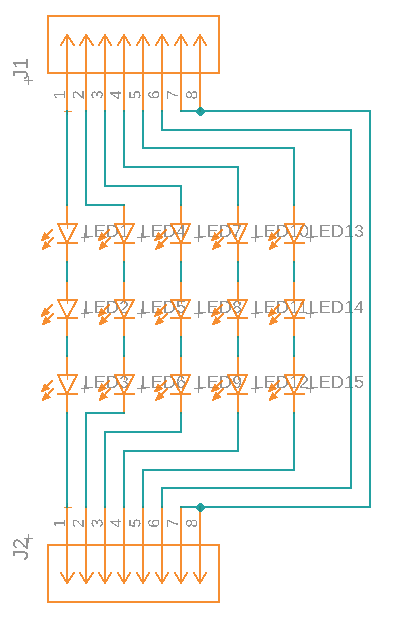
\includegraphics[width=\textwidth]{../assets/schematics/lighting_led_sch.png}}
        \caption{Schematic.}
        \label{fig:lighting_led_sch}
      \end{subfigure}
      \hspace{.08\textwidth}
      \begin{subfigure}{.35\textwidth}
        \centering
        \frame{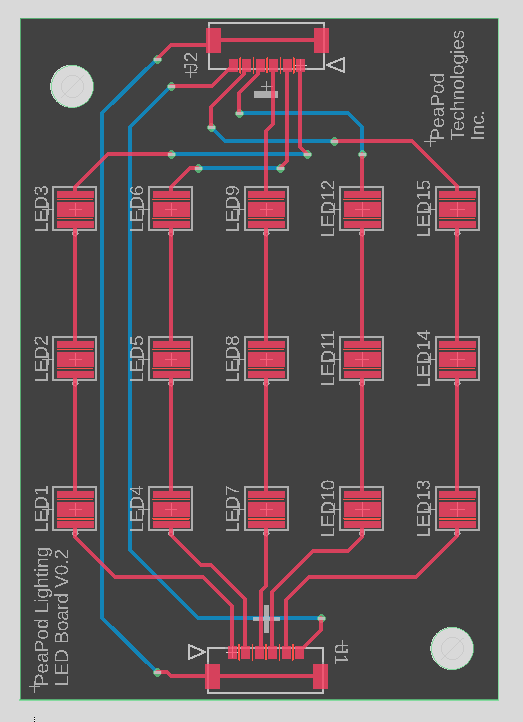
\includegraphics[width=\textwidth]{../assets/schematics/lighting_led_brd.png}}
        \caption{PCB layout.}
        \label{fig:lighting_led_brd}
      \end{subfigure}
      \caption{Lighting LED board.}
\end{figure}

\begin{figure}[h!]
    \centering
    \begin{subfigure}{.35\textwidth}
        \centering
        \frame{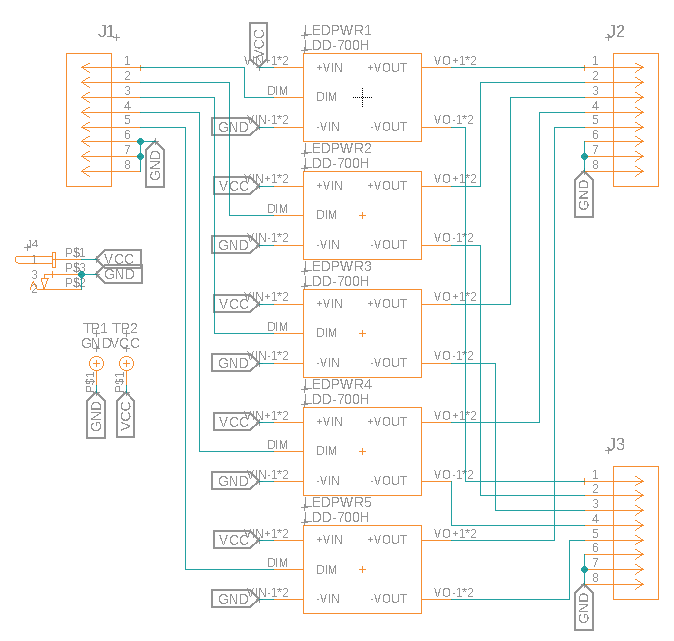
\includegraphics[width=\textwidth]{../assets/schematics/lighting_power_sch.png}}
        \caption{Schematic.}
        \label{fig:lighting_power_sch}
      \end{subfigure}
      \hspace{.02\textwidth}
      \begin{subfigure}{.6\textwidth}
        \centering
        \frame{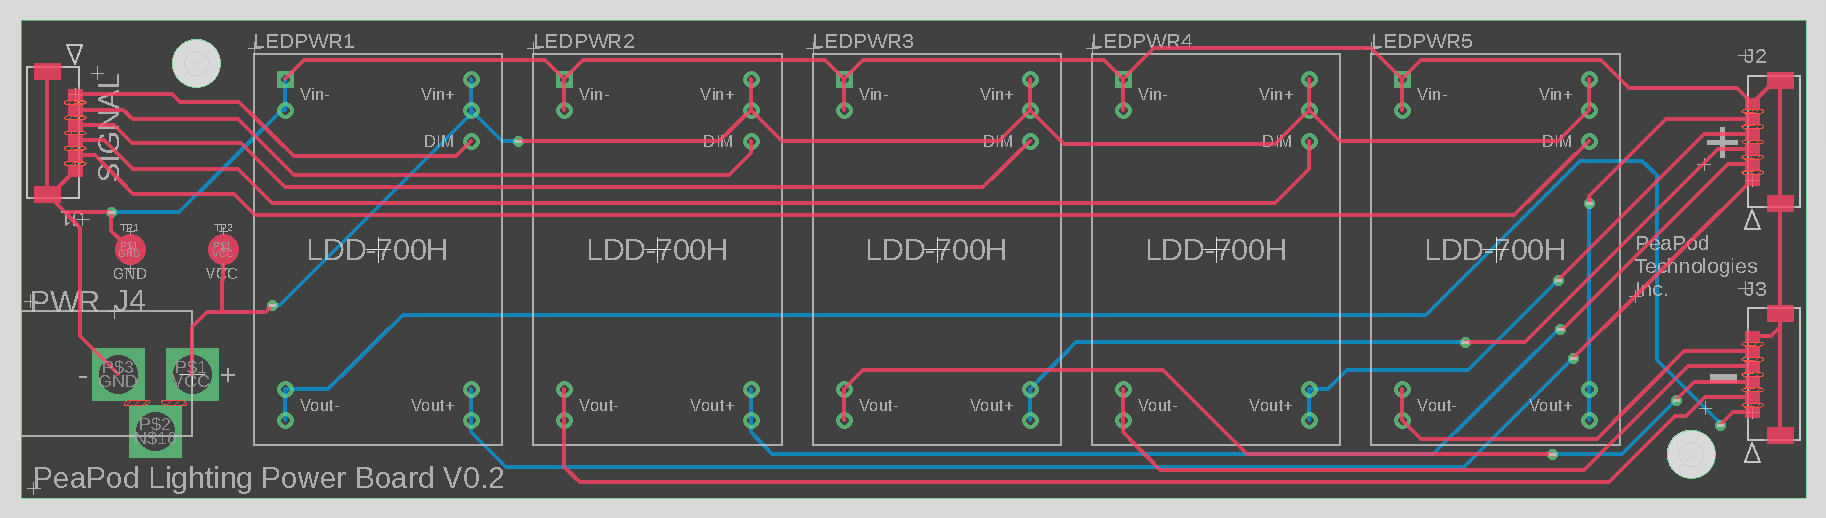
\includegraphics[width=\textwidth]{../assets/schematics/lighting_power_brd.png}}
        \caption{PCB layout.}
        \label{fig:lighting_power_brd}
      \end{subfigure}
      \caption{Lighting power board.}
\end{figure}

\clearpage

\subsection{Optimization}
\label{sec:optimization}

\textbf{Purpose}: Iteratively improve yield, etc. of crops as more environment condition and plant metric data is gathered across different programs over multiple growth cycles.

\textbf{Function}:
\begin{itemize}
    \item \textbf{Inputs}: Growth cycle datasets (Environment data across time (control system portion of $\vec E(t)$), plant performance metric (PPM) data across time ($\vec P(t)$), associated program (actuated portion of $\vec E(t)$))
    \item \textbf{Outputs}: Plant-program performance prediction model, novel programs
\end{itemize}

\textbf{Method}: 

Assume a plant's growth rate (or state change) is related to its current internal state $\vec P \in \R^n$ (for $n$ plant metrics) and the environment conditions $\vec E \in \R^m$ (for $m$ environment parameters). Let these both be functions $\vec P (t),\vec E(t)$ defined at each $t$, where $t=0$ indicates the time of planting. Assume that this relationship is constant for all members of a given species.

Define plant state change $\vec P'$: 

$$\vec P'(t) = \frac{d}{dt}\vec P(t)$$

Define the plant-environment behaviour function $Q$: 

$$Q(\vec P(t), \vec E(t), t)=\vec P'(t)$$ 

Given the current internal and external states, determine the plant's state change.

\begin{enumerate}
    \item Set $\vec E_{set}(t)~\forall~ t$, aka the program (\ref{sec:automation});
    \item Record $\vec P(t)~\forall~ t$ and $\vec E(t)\approx \vec E_{set}(t)~\forall~ t$;
    \item Calculate $\vec P'(t)~\forall~ t$;
    \item Fit $\vec Q$ to our data;
\end{enumerate}

By fitting $\vec Q$ across iterations, we can predict $\vec P$ at any $\vec E$ and $t$. For example:

$$\vec P(t+\Delta t)=P(t)+\Delta t\cdot Q(\vec P(t),\vec E(t))$$

Gradient ascent with this model can be used to generate novel (theoretically improved) programs.

\textbf{Features}:
\begin{itemize}
    \item \textit{Machine Learning Model}: Represented by $Q$. Operates in the cloud.
    \item \textit{Environment Data} (over time): Represented by $\vec E(t)$. Collected by sensors (for \textit{control loop} environment parameters) and extracted from the associated program (for \textit{actuated instruction} environment parameters). See Section \ref{sec:automation}.
    \item \textit{PPM Data} (over time): Represented by $\vec P(t)$. Extracted from computer vision. See Section \ref{sec:automation}.
\end{itemize}

\clearpage

% \section{System-Level Build Process Report}
% % System-level report (i.e. block diagram) of build process

% \subsection{Materials}
\subsubsection{System}

\textbf{Automation}\\

\begin{table}[!h]
    \centering
    \begin{tabular}{|c|l|l|l|c|}
    \hline
        Index   & Manufacturer Part Number  & Manufacturer Name         & Description                       & Quantity  \\ \hline
        1       & A000005                   & Arduino                   & ARDUINO NANO ATMEGA328 EVAL BRD   & 1         \\ \hline
        2       & S404GSEJ6-U3000-3         & Delkin Devices, Inc.      & 4GB MLC MICROSD CARD (-25C - +85  & 1         \\ \hline
        3       & 61304021121               & Würth Elektronik          & CONN HEADER VERT 40POS 2.54MM     & 1         \\ \hline
        4       & SC0510                    & Raspberry Pi              & ZERO 2 W                          & 1         \\ \hline
        5       & DMN2005K-7                & Diodes Incorporated       & MOSFET N-CH 20V 300MA SOT23-3     & 2         \\ \hline
        6       & RC0603FR-0710KL           & YAGEO                     & RES 10K OHM 1\% 1/10W 0603        & 5         \\ \hline
        7       & 4484                      & Adafruit Industries LLC   & MINI PITFT 1.3 FOR RASPBERRY PI   & 1         \\ \hline
        8       & 5055670271                & Molex                     & CONN HEADER SMD R/A 2POS 1.25MM   & 2         \\ \hline
        9       & 5055670471                & Molex                     & CONN HEADER SMD R/A 4POS 1.25MM   & 5         \\ \hline
        10      & 5055670871                & Molex                     & CONN HEADER SMD R/A 8POS 1.25MM   & 3         \\ \hline
        11      & 5055670681                & Molex                     & CONN HEADER SMD R/A 6POS 1.25MM   & 3         \\ \hline
    \end{tabular}
    \caption{Automation system electronic components.}
    \label{tab:automation_components}
\end{table}

In addition, 1x \textit{Automation Motherboard PCB}: 2 Layers, 1 oz. Copper, 1.6mm Thickness, Suggested: HASL Finish (Lead-Free), White PCB, Black Silkscreen

\textbf{Housing}\\

\begin{table}[!ht]
    \centering
    \begin{tabular}{|l|l|c|l|l|}
    \hline
        Part                    & Description                                           & Quantity  & Supplier          & Supplier Part Number  \\ \hline
        Control Module Housing  & 5-Sided enclosure                                     & 1         & Protocase         & ~                     \\ \hline
        Frame Front X Extrusion & Silver Painted, 20x20mm, Ordered 2ft., Cut to 500mm   & 2         & McMaster-Carr     & 5537T101              \\ \hline
        Frame Door Y Extrusion  & Silver Painted, 20x20mm, Ordered 2ft., Cut to 500mm   & 2         & McMaster-Carr     & 5537T101              \\ \hline
        Frame Rear X Extrusion  & Silver Painted, 20x20mm, Ordered 2ft., Cut to 460mm   & 2         & McMaster-Carr     & 5537T101              \\ \hline
        Frame Door X Extrusion  & Silver Painted, 20x20mm, Ordered 2ft., Cut to 460mm   & 2         & McMaster-Carr     & 5537T101              \\ \hline
        Frame Rear Y Extrusion  & Silver Painted, 20x40mm, Ordered 2ft., Cut to 460mm   & 2         & McMaster-Carr     & 5537T111              \\ \hline
        Frame Front Y           & Silver Painted, 20x20mm, Ordered 2ft., Cut to 460mm   & 2         & McMaster-Carr     & 5537T101              \\ \hline
        Frame Z                 & Silver Painted, 20x20mm, Ordered 2ft., Cut to 460mm   & 4         & McMaster-Carr     & 5537T101              \\ \hline
        Tray X Extrusion        & Silver Painted, 20x20mm, Ordered 2ft., Cut to 440mm   & 4         & McMaster-Carr     & 5537T101              \\ \hline
        Tray Z Extrusion        & Silver Painted, 20x20mm, Ordered 2ft., Cut to 400mm   & 6         & McMaster-Carr     & 5537T101              \\ \hline
        Nozzle Arm Extrusion    & Silver Painted, 20x20mm, Ordered 1ft., Cut to 150mm   & 2         & McMaster-Carr     & 5537T101              \\ \hline
        M5x0.8 10mm Bolts       & Alloy Steel, Black Oxide Coated, Socket Head Cap      & 139       & McMaster-Carr     & 91290A224             \\ \hline
        M5x0.8 16mm Bolts       & Alloy Steel, Black Oxide Coated, Socket Head Cap      & 10        & McMaster-Carr     & 91290A232             \\ \hline
        M4x0.7 16mm Bolts       & Alloy Steel, Black Oxide Coated, Socket Head Cap      & 12        & McMaster-Carr     & 91290A154             \\ \hline
        M4x0.7 Hex Nuts         & High-Strength Steel, Black Oxide Coated               & 12        & McMaster-Carr     & 94166A110             \\ \hline
        M5 T-Nuts               & Zinc-Plated Steel, Black Painted, for 5mm Slot        & 139       & McMaster-Carr     & 5537T651              \\ \hline
        M5x0.8 Hex Nuts         & Alloy Steel, Black Oxide Coated                       & 10        & McMaster-Carr     & 94166A120             \\ \hline
        Foam Insulation         & DUROSPAN GPS R5 4ft. x 8ft. x 1in.                    & 1         & Home Depot Canada & 1001211234            \\ \hline
        Reflective Mylar        & 27in. x 12ft. x 0.002in., Aluminum-coated PET         & 1         & McMaster-Carr     & 7538T11               \\ \hline
        Adhesive                & LePage PL300 Foamboard 295mL                          & 2         & Home Depot Canada & 1000403469            \\ \hline
        Grow Cup                & 2in. Diameter                                         & 16        & Amazon            & ~                     \\ \hline
        Door Hinges             & Plastic, Black, for 20x20mm Extrusion                 & 2         & McMaster-Carr     & 5537T85               \\ \hline
        Feet Bumpers            & Adhesive-Back, Medium-Hard Polyurethane, Black        & 4         & McMaster-Carr     & 95495K24              \\ \hline
    \end{tabular}
    \caption{Housing subsystem components.}
    \label{tab:housing_parts}
\end{table}

\begin{table}[!ht]
    \centering
    \begin{tabular}{|l|c|l|l|}
    \hline
        Part                        & Quantity  & Materials             & Process           \\ \hline
        L Bracket                   & 12        & PETG Filament         & 3D Printing       \\ \hline
        L Bracket (Grow Tray)       & 4         & PETG Filament         & 3D Printing       \\ \hline
        Diagonal Bracket            & 4         & PETG Filament         & 3D Printing       \\ \hline
        T Bracket                   & 10        & PETG Filament         & 3D Printing       \\ \hline
        Tray Hook BL                & 2         & PETG Filament         & 3D Printing       \\ \hline
        Tray Hook BR                & 2         & PETG Filament         & 3D Printing       \\ \hline
        Tray Hook FL                & 2         & PETG Filament         & 3D Printing       \\ \hline
        Tray Hook FR                & 2         & PETG Filament         & 3D Printing       \\ \hline
        Grow Plate Quarters         & 4         & 210x210x5mm PET Sheet & Table Saw         \\ \hline
        Grow Plate Washer           & 1         & PETG Filament         & 3D Printing       \\ \hline
        Nozzle Mount A              & 2         & PETG Filament         & 3D Printing       \\ \hline
        Nozzle Mount B              & 2         & PETG Filament         & 3D Printing       \\ \hline
        Lighting LED Board Mount    & 5         & PETG Filament         & 3D Printing       \\ \hline
        Lighting Power Board Mount  & 1         & PETG Filament         & 3D Printing       \\ \hline
        Feet                        & 4         & PETG Filament         & 3D Printing       \\ \hline
    \end{tabular}
    \caption{Housing subsystem fabricated parts.}
    \label{tab:housing_fabrication}
\end{table}

\textbf{Aeroponics}\\


\textbf{Leaf-Zone Thermoregulation}\\


\textbf{Humidification}\\


\textbf{Dehumidification}\\


\textbf{Gas Composition Regulation and Exchange}\\


\textbf{Lighting}\\


\subsubsection{Inputs}
% Supply inputs (water, power, network), consumable inputs (pH/nutrient solutions, dehumidification cartridge)

\textbf{Supply Inputs}
\begin{itemize}
    \item \textit{Water}: reverse-osmosis, ambient
    \item \textit{Power}: 120V 60Hz AC\footnote{The power supply can be altered to suit a variety of power inputs (i.e. DC)}
    \item \textit{Network}: ethernet or wireless, optional
\end{itemize}

\textbf{Consumable Inputs}
\begin{itemize}
    \item \textit{Nutrient/pH Adjusment Solutions}: pouches
    \item \textit{Dehumidification Cartridge}: recharged
\end{itemize}

\subsubsection{Outputs}
% Food outputs(?), by-products/waste (waste water from flushing, dehumidification cartridge)

\textbf{Food Outputs}\\


\textbf{By-Products \& Waste}\\


\subsubsection{Maintenance}

\textbf{Spare Components}\\


\textbf{Tools}\\


\subsubsection{Cleaning}

\textbf{Soaps}\\


\textbf{Disinfectants}\\


\textbf{Tools}\\



\section{Prototype Build Status}
% SPECIFICALLY build status - from functional prototyping to testing to refinement

\subsection{Completion}
The prototype is 50\% complete as of May 31st, 2022. The housing, aeroponics supply system (without dosage pumps or thermoregulation), lighting, and automation systems are fully operational.


\subsection{Successes, Results, and Products}
% Please describe any successes (e.g. preliminary results) and predicted and/or produced food outputs

As of May 31st, 2022, no food has been produced by PeaPod. However, we predict successful production of a variety of plant-based food products over the coming weeks, derived from a variety of plant types (leafy greens, legumes, garden vegetables, microgreens, root vegetables, herbs) and prepared using a variety of methods and combinations (i.e. meals). This is possible despite prototype incompleteness, as the remainder of subsystems (except nutrient/pH adjustment solution dosage) are non-critical to plant growth when ambient temperature, humidity, and gas composition are relatively suitable for plant growth at typical indoor ambient atmospheric conditions. In addition, this will still produce usable data for optimization, as all sensors are in place and collecting data even though their associated control systems are absent.

\uline{\textbf{835 Characters} (5000 max)}

\subsection{Challenges}
% Please describe any challenges that you have encountered in developing your design and/or prototype since Phase 1.

Processes for pollination and germination are still unclear, though simple solutions are possible (air circulation for pollination, seed planting/germination in-place).

Due to the high current draw of the Peltier device (8.5A), as well as the necessity of voltage control over PWM, a custom driver circuit needed to be designed (as opposed to an off-the-shelf integrated circuit). The multi-stage driver (PWM to step-up MOSFETs to low-pass filter to operational amplifier voltage buffer to Darlington amplifier with feedback to relay H-bridge) was non-intuitive to design, and required many revisions (choosing Darlington over MOSFET due to op amp output current limits, choosing relays over MOSFETs due to variable supply voltage).

Specific component placement and orientation for extended housing topologies (as well as the process of actually extending a housing) is still unclear.

Selection of an aeroponics system type was a key design challenge, specifically around the ability to deliver mineral-rich water without calcification at high water delivery rates with suitable droplet diameter, which ultimately led to our selection of high-pressure nozzle-based aeroponics over piezoelectric mesh nebulizer aeroponics (as is used in some commercial settings).

Initially, the method of nutrient and pH-adjustment solution injection was Venturi siphon based. This presented a number of key issues, mainly controlling injection rate/mixing proportions while preventing backflow under pressure, which led us to pivot to peristaltic pumps, which have proven to be superior in both aspects.

\clearpage

The lighting system PCBs went through 4 revisions before consistently successful functionality was achieved. Reasons include pin alignment during LED board daisy-chaining, thermal management, and LED power limits.

The fitting selection for the aeroponics supply system was fully redesigned twice, first because of new component selection, and then again for part count/mass optimization. The aeroponics supply system also leaked frequently prior to optimizing the assembly process (proper securing of tapered and parallel thread mating faces using PTFE tape and bonded O-rings, respectively, as well as proper tightening).

The software has been restructured and portions completely rewritten countless times. Establishing and maintaining reliable computer-microcontroller communications over serial was challenging, as we did not initially realize that the two devices' IO operated at different voltages (3.3V vs 5V, respectively). Ensuring message validity (JSON formatting, delimiters, encoding, etc.) was also difficult, and was ultimately solved by writing unit testing suites for both devices' communication software. In addition, being able to flash microcontroller firmware from the computer on the fly required a number of revisions. 

Cloud communication was also a major challenge, as registering an IoT device with an API required keypair generation. Manual/hard-coded keypairs are not user-friendly or particularly secure, and a cryptographic integrated circuit built into the motherboard goes against our open-source mission. We ultimately settled on the following process: the user securely enters their credentials for an authentication provider (Google, GitHub, Microsoft, etc.) using the OAuth Device Flow method, and the device "logs in" to our API as the user. The device can then request a private key from our API, which generates the keypair (supposing the user has not exceeded their device quota) and stores the public key on the backend. The device has effectively "self-registered", and can publish data and recieve live config data autonomously.

For a long time, the aeroponic container was a "black box" in our design, meaning that we had no idea where to even begin. One of our team members suggested tent material, and prototyping took off once we found the specific composite that met our requirements (high strength/low weight, fully waterproof, no coating/food-safe, relatively easy to assemble). Assembling the container required a number of iterations, as we initially overlooked the additional material needed for seams (fused with pressure-sensitive adhesive) when calculating the dimensions, as well as choosing a variant of the composite fabric that was too thin and ultimately developed microtears.

Logistical issues also presented themselves during the prototyping process. We had to move locations twice, and our primary 3D printer spontaneously broke.

Currently, the custom peristaltic dosage pumps are being prototyped. This requires tight tolerances in 3D printing, due to the specific mechanism of peristalsis (pump housing not tight enough, tubing does not fully shut under force from the rollers and water is able to backflow through the pump; pump housing is too tight, and the tubing wears out very quickly, or the rollers don't move at all, overheating the stepper motor). In addition, the thermoregulation systems (both leaf- and root-zone) are nearing completion, with only heat sink selection and subsystem testing remaining.

\uline{\textbf{5108 Characters} (5000 max)}

\clearpage

\subsection{Timeline}
% What are your next steps? Incl. estimated completion date

% maximum 5000 characters

The timeline as of May 31st 2022 is as follows:
\begin{itemize}
    \item \textit{June 2022}: Finish design. Continue prototyping. Grow our first plants and collect data.
    \item \textit{July 2022}: Complete prototype. Assemble and distribute prototypes to schools and volunteers for beta testing, publicly sharing collected data and diagnostic information. Make design/prototype improvements based on beta testing. Begin constructing the optimization machine learning model.
    \item \textit{August 2022}: Collect samples for nutritional and safety analysis. Collaborate globally on distributed phenological research. Publish findings.
\end{itemize}

Estimated latest prototype completion date: \textbf{August 1st, 2022}.

\clearpage

\section{Prototype Progress}
% To be extracted as a separate PDF and submitted as 2.5

\subsection{Automation}
\label{sec:automation}

\textbf{Purpose}: Performing growth-, maintenance-, and data-related tasks autonomously on the basis of both schedule and necessity to reduce crew maintenance time, improve consistency of products, and eliminate safety risks. Maintains the homogeneity of the internal environment with increased accuracy and precision over crew interference, while enabling simultaneous control over all parameters.

\textbf{Function}:
\begin{itemize}
    \item \textbf{Inputs}: Environment data stream (sensor readings), growth program
    \item \textbf{Outputs}: Actuator control signals, crew/cloud messaging, environment data (stored), timelapse photo set
\end{itemize}

\textbf{Method}:
\begin{enumerate}
    \item \textit{Setup}:
    \begin{enumerate}
        \item Power is connected and system is booted;
        \item Program is selected by user;
    \end{enumerate}
    \item \textit{Testing}:
    \begin{itemize}
        \item Power-on Self-Test (POST) passes (i.e. all hardware is online and communicating as expected).
        \item Systems enact program as intended (i.e. control systems respond properly).
    \end{itemize}
    \item \textit{Process}:
    \begin{enumerate}
        \item Checks operating preconditions (self POST and per-subsystem);
        \item \textbf{Environment Control Loop} (matches \textit{Sense-Plan-Act} model of robotics): %TODO cite the model
        \begin{enumerate}
            \item \textit{Sense}: Receives and stores data about current environment state;
            \item \textit{Plan}: Compares current state to "desired"/program state, develops a "plan"/actuator control to reach desired state;
            \item \textit{Act}: Controls subsystem operations in order to enact the plan;
        \end{enumerate}
        \item Notifies user on maintenance requirement (i.e. non-automated input/output management, refills, repairs, etc.), end-of-program (EoP), and diagnostic info;
    \end{enumerate}
    \item \textit{Shutdown} (either manual or EoP):
    \begin{enumerate}
        \item Stop all subsystem operations;
        \item Power down;
    \end{enumerate}
\end{enumerate}

\clearpage

\textbf{Features}:

A dual-computer system was chosen to allow for discrete management of high-level functionality (camera capture, internet/cloud functionality, local storage, complex calculations, etc.) and low-level functionality (hardware-level communications, actuator control and GPIO) in a master/slave topology with a constant two-way stream of shared data.

\begin{itemize}
    \item \textit{Computer (Master)} \cite{raspberrypi}: Manages data collection, batch storage, analysis, and transmission/receiving, as well as planning/calculations for actuator control. Includes internal clock (for program, notification), network connection (for data transmission, notification), photo capture, and non-volatile storage (for data/photos). Sends instructions derived from the program to the microcontroller.
    \item \textit{Microcontroller (Slave)} \cite{arduino}: Manages detailed sensor/actuator states and communications (on/off, sensor readings, actuator control). Streams collected sensor readings to the computer.
    \item \textit{Program}: Set of actuated instructions (e.g. lights on) and control targets (e.g. hold air temperature at 22°C) to enact at specific points in the growth cycle, as well as config data;
    \item \textit{Camera Capture \& Plant Performance Metric (PPM) Extraction}: Top-down and side-view cameras \cite{camera}, captured under standard lighting at regular intervals throughout the course of the growth cycle. For live feed transmission to users (local and remote), as well as PPM extraction via computer vision and machine learning for yield and diagnostic analysis. Potentially relevant PPMs include (but are not limited to):
    \begin{itemize}
        \item Leaf health indicators (i.e. leaf tip burn, leaf curl, chlorosis);
        \item Leaf count, size distribution;
        \item Leaf density;
        \item Canopy dimensions/surface area;
        \item Plant height;
        \item Fruit/harvest body size, ripeness;
    \end{itemize}
    \item \textit{Environment Data}: Record the environment's current state. Covers each \textit{control system} environment parameter (e.g. included in a feedback loop). Control system environment parameters include:
    \begin{itemize}
        \item Leaf-zone temperature (see \ref{sec:airthermoregulation});
        \item Leaf-zone humidity (see \ref{sec:humidityregulation});
        \item Root-zone temperature (see \ref{sec:aeroponics});
        \item Gas concentrations (see \ref{sec:gas});
    \end{itemize}
    \item \textit{Actuator Control}: Induces change in environment parameters. Covers both \textit{control system} and \textit{actuated instruction} environment parameters. Actuated instruction environment parameters include:
    \begin{itemize}
        \item Lighting (see \ref{sec:lighting});
        \item Water delivery (see \ref{sec:aeroponics});
        \item Plant nutrient delivery (see \ref{sec:aeroponics});
        \item Water pH (see \ref{sec:aeroponics});
        \item Air circulation rate (see \ref{sec:airthermoregulation});
    \end{itemize}
    \item \textit{Diagnostic Systems}: Include informative sensors tracking system input availability, subsystem diagnostics, etc. as well as notification triggers.
\end{itemize}

\clearpage

\textbf{Figures}

\begin{figure}[h!]
    \centering
    \frame{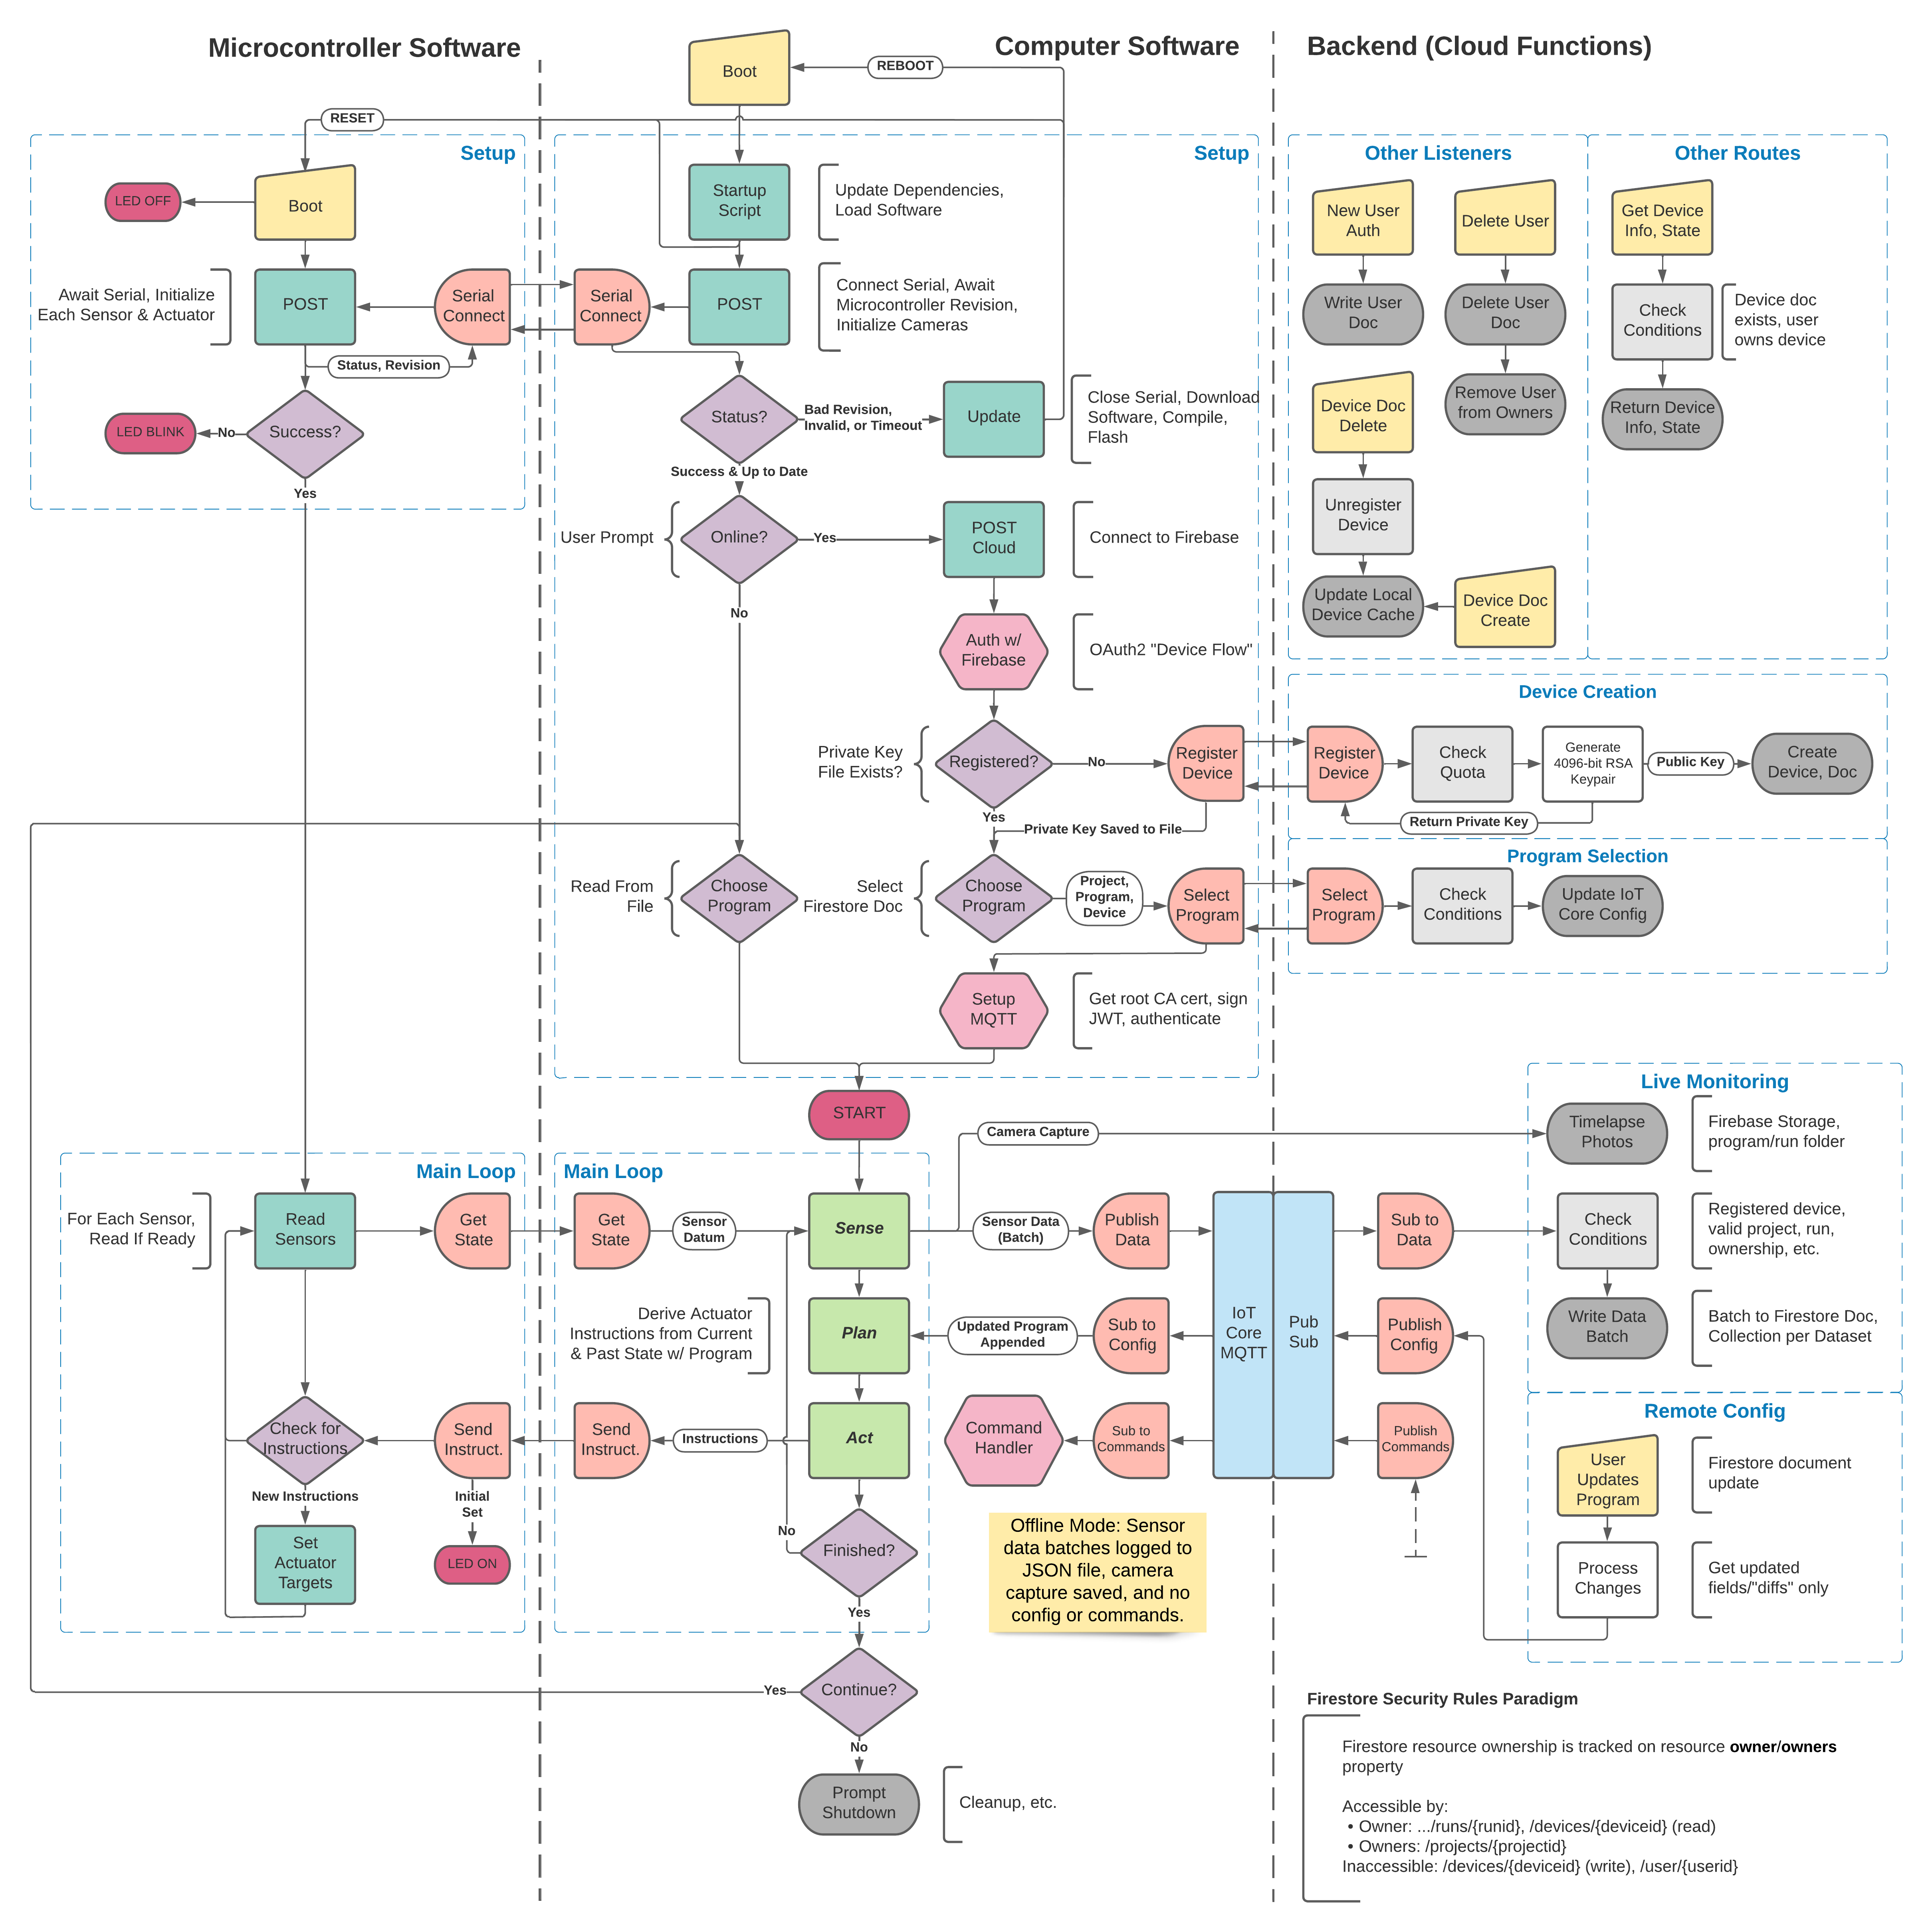
\includegraphics[width=\textwidth]{../assets/figures/automation_software.png}}
    \caption{Software control flow diagram.}
    \label{fig:automation_software}
\end{figure}

\begin{figure}[h!]
    \centering
    \frame{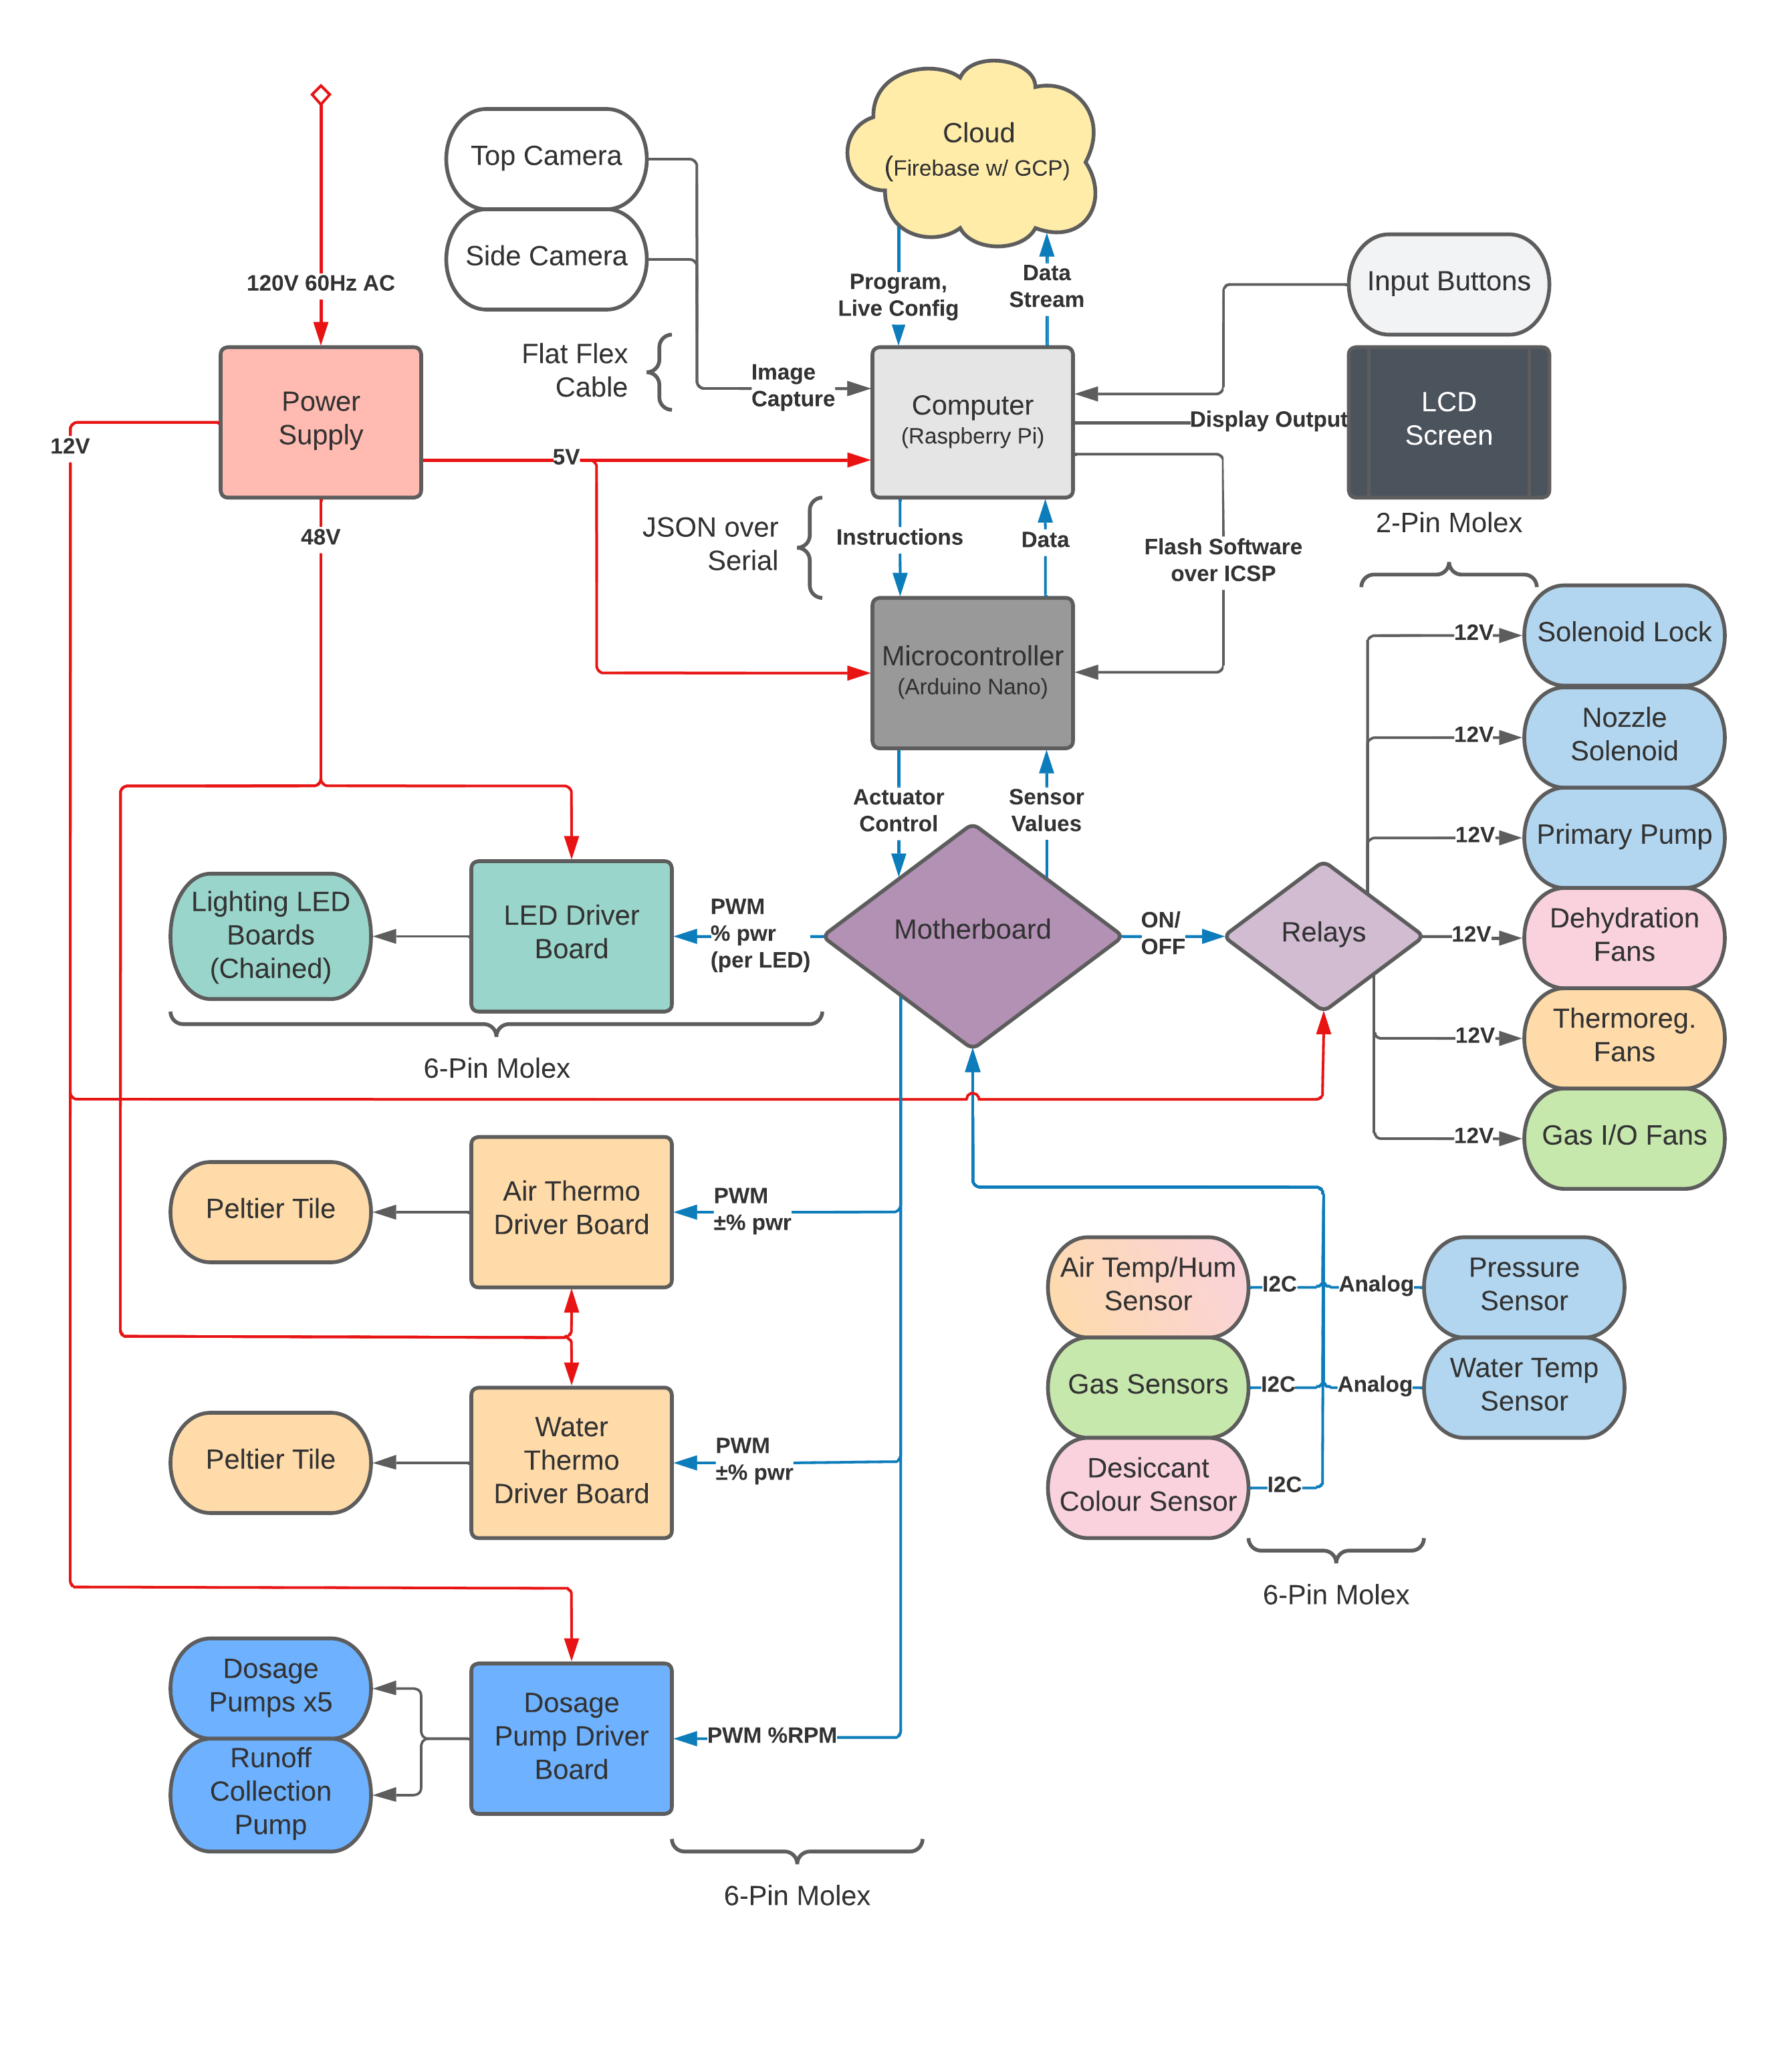
\includegraphics[width=\textwidth]{../assets/figures/automation_wiring.png}}
    \caption{System wiring diagram.}
    \label{fig:automation_wiring}
\end{figure}

\clearpage

\subsection{Housing}

\begin{figure}[h!]
  \centering
  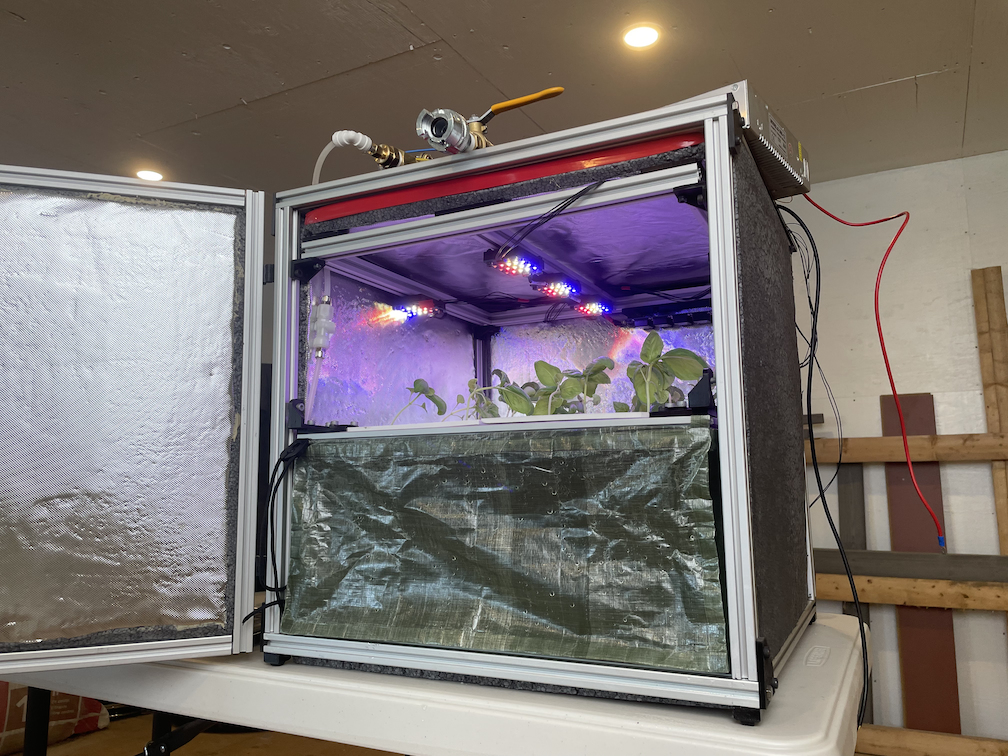
\includegraphics[width=\textwidth]{../assets/photos/prototype_housing.png}
  \hfill
  \caption{Housing prototype. Note lighting and grow trays, as well as reflective sheet-laminated foam insulation panels.}
  \label{fig:prototype_housing}
\end{figure}

The prototype performs all functions as designed.

\clearpage

\subsection{Aeroponics}
\label{sec:aeroponics}

\textbf{Purpose}: Delivers plant nutrients and pH- and temperature-controlled water to the roots via a fine mist.

\textbf{Function}:
\begin{itemize}
    \item \textbf{Inputs}: Reverse osmosis water\footnote{RO water has no dissolved nutrients and a neutral pH of 7.0. This enables easier and more reliable calculations. In addition, it has no particulate or minerals, minimizing the chances of nozzle clog.} under positive pressure, concentrated pH up \& down solutions and nutrient solutions, nozzle delivery on/off control (\ref{sec:automation}), pH and nutrient solution ratios as control signals (dosing pump speeds; \ref{sec:automation}), water thermoregulation control signal (\ref{sec:automation})
    \item \textbf{Outputs}: pH- and nutrient-controlled water mist (50 micron mean droplet diameter)
\end{itemize}

\textbf{Method}:
\begin{enumerate}
    \item \textit{Setup}:
    \begin{enumerate}
        \item Hook up water, solution, and signal inputs;
        \item Connect the quick-disconnect fitting;
        \item Calibrate pressure, temperature sensors to atmospheric;
        \item Enable water input to prime system (if known pressure/temperature, calibrate sensors);
        \item Mount container, connect runoff collection line to recycling port;
    \end{enumerate}
    \item \textit{Testing}:
    \begin{itemize}
        \item Temperature, pressure sensors communicate as expected;
        \item No leaks at any connections under a) source pressure, b) fully pressurized;
        \item Pump actuates and auto-shuts off as expected, and is able to deliver the required pressure;
        \item All components, tubing, and connectors/fittings withstand full pressurization;
        \item Solenoid is normally closed, withstands full pressurization, and opens when power is applied;
        \item Quick-disconnect operates as intended at full pressurization without leaks;
        \item Nozzles produce even-distribution full-cone mist;
        \item Manual and actuated valves operate as intended;
        \item Runoff container is sealed, and runoff collection operates as intended;
    \end{itemize}
    \item \textit{Process}:
    \begin{enumerate}
        \item Water is pressurized to constant 80psi;
        \item Heat is added to or removed from the water;
        \item Temperature and pressure of the water is read (feedback);
        \item Nutrient and pH solutions are mixed in-line at an adjustable ratio\footnote{I.e. add X mL of nutrient solution Y per mL water to achieve Z ppm, or add A mL of pH down solution per mL water to achieve a pH of B.};
        \item Flow to nozzle is controlled (on/off);
        \item Nozzle turns pressurized water into mist;
        \item Runoff is contained by a water-tight container, and collected for recycling;
    \end{enumerate}
    \clearpage
    \item \textit{Shutdown}:
    \begin{enumerate}
        \item Power down the pump and thermoregulation unit;
        \item Close the nutrient and pH solution valves;
        \item Close the source shutoff valve;
        \item Open the drain valve, and allow the system to depressurize completely;
        \item Re-open the source shutoff valve and flush the system with fresh water;
        \item Power down the solenoid;
        \item Collect all remaining runoff;
        \item Disconnect the quick-disconnect fitting;
        \item Disconnect the inputs;
    \end{enumerate}
\end{enumerate}

\textbf{Features}:
\begin{itemize}
    \item \textit{Water Source}: Input for ambient reverse-osmosis water.
    \item \textit{Manual Source Shutoff Valve}: Ball valve.
    \item \textit{Diaphragm Pump}: Self-priming, auto-shutoff at 80psi. Power is controlled by a relay.
    \item \textit{Inline Thermoelectric Water Heater/Cooler Block}: Aluminum water block heat pump. See Section \ref{sec:airthermoregulation}.
    \item \textit{PID Control Loop}: A propotional-integral-derivative control loop enables increased accuracy (see equation \ref{eqn:pid}, \ref{sec:airthermoregulation}).
    \item \textit{Solution Injection Manifold}: A manifold of parallel inline injectors, allowing for on-demand adjustment of mixing ratios for nutrient and pH solutions. Comprises:
    \begin{itemize}
        \item \textit{Manifold}: Splits the water line into a set of parallel branches with inline tees to enable solution injection.
        \item \textit{Dosing Pumps}: Stepper-motor driven custom peristaltic pumps deliver solutions at a controlled rate/ratio (one per solution). Toleranced to prevent backflow at pressure. % TODO more details (tubing type, washers, bearings, etc.) w/ part numbers
        \item \textit{Nutrient Solutions}: Aqueous. Highly concentrated. Selectable as part of the program (\ref{sec:automation})\footnote{Many different solutions can be combined (according to solubility laws, pH requirements, etc.).}, and may include any of:
        \begin{itemize}
            \item Bioavailable nonmetals (ammonia, ammonium, nitrates, nitrites, phosphates, sulfates, etc.)
            \item Bioavailable metals (potassium, etc.)
            \item Minerals (magnesium, calcium)
            \item Other trace elements
            \item Custom solutions (i.e. fungicides/algicides, descaling solutions)
        \end{itemize} 
        \item \textit{pH Adjustment Solutions}\footnote{\textit{NOTE:} Ionic composition of pH solutions should be considered in the understanding of the nutrient composition (i.e. phosphic acid results in phosphate ions in spray)}: Aqueous. Highly concentrated. One for pH up (>8), one for pH down (<6).
        \item \textit{Solution Storage Containers}: Opaque, insulated, chemical-safe, refillable cartridges. Prevent degradation of solution compounds over time via light or heat.
        \begin{itemize}
            \item \textit{Fill Level Sensors}: Depth sensors measure fill level of container. Notifies user to refill.
        \end{itemize}
    \end{itemize}
    \item \textit{Water Temperature Sensor}: Tee-fitted. Informs a \textbf{PID control loop}. See Section \ref{sec:airthermoregulation}.
    \item \textit{Accumulator Tank}: Uses an air bladder to maintain and stabilize pressure.
    \item \textit{Pressure Sensor}: Allows for shutoff of pump in case of emergency.
    \item \textit{Drain Valve}: Tee-fitted ball valve. Allows the system to be depressurized and drained.
    \item \textit{Solenoid Valve}: Controls delivery to the nozzles to enable on-demand misting.
    \item \textit{Grow Tray Quick-Disconnect}: Connectors between aeroponics supply and nozzles that allow for quick disconnection with auto-shutoff so the trays may be removed.
    \item \textit{Nozzle}: Mounted to grow tray, pointed at plant roots. 80psi water through a 0.4-0.6mm orifice produces 5-50 micron water droplets, optimal for plant growth. This method is 98\% more water-efficient than traditional farming.%TODO: Sources??
    \item \textit{Root-Zone Container}: Watertight container that encapsulates the entire root zone. Made of a woven waterproof composite fabric (CT5K.18 mylar with Dyneema, 1.43oz/yd${}^2$ or 33.89g/m${}^2$), chosen for high strength-to-weight ratio (15x that of steel) and natural no-coating food-safe waterproof quality \cite{dyneema}. Mounted and \textbf{sealed} to the grow tray with a drawstring for easy root zone access. Provides water supply and runoff collection ports.
\end{itemize}

\textbf{Figures}

\begin{figure}[h!]
    \centering
    \frame{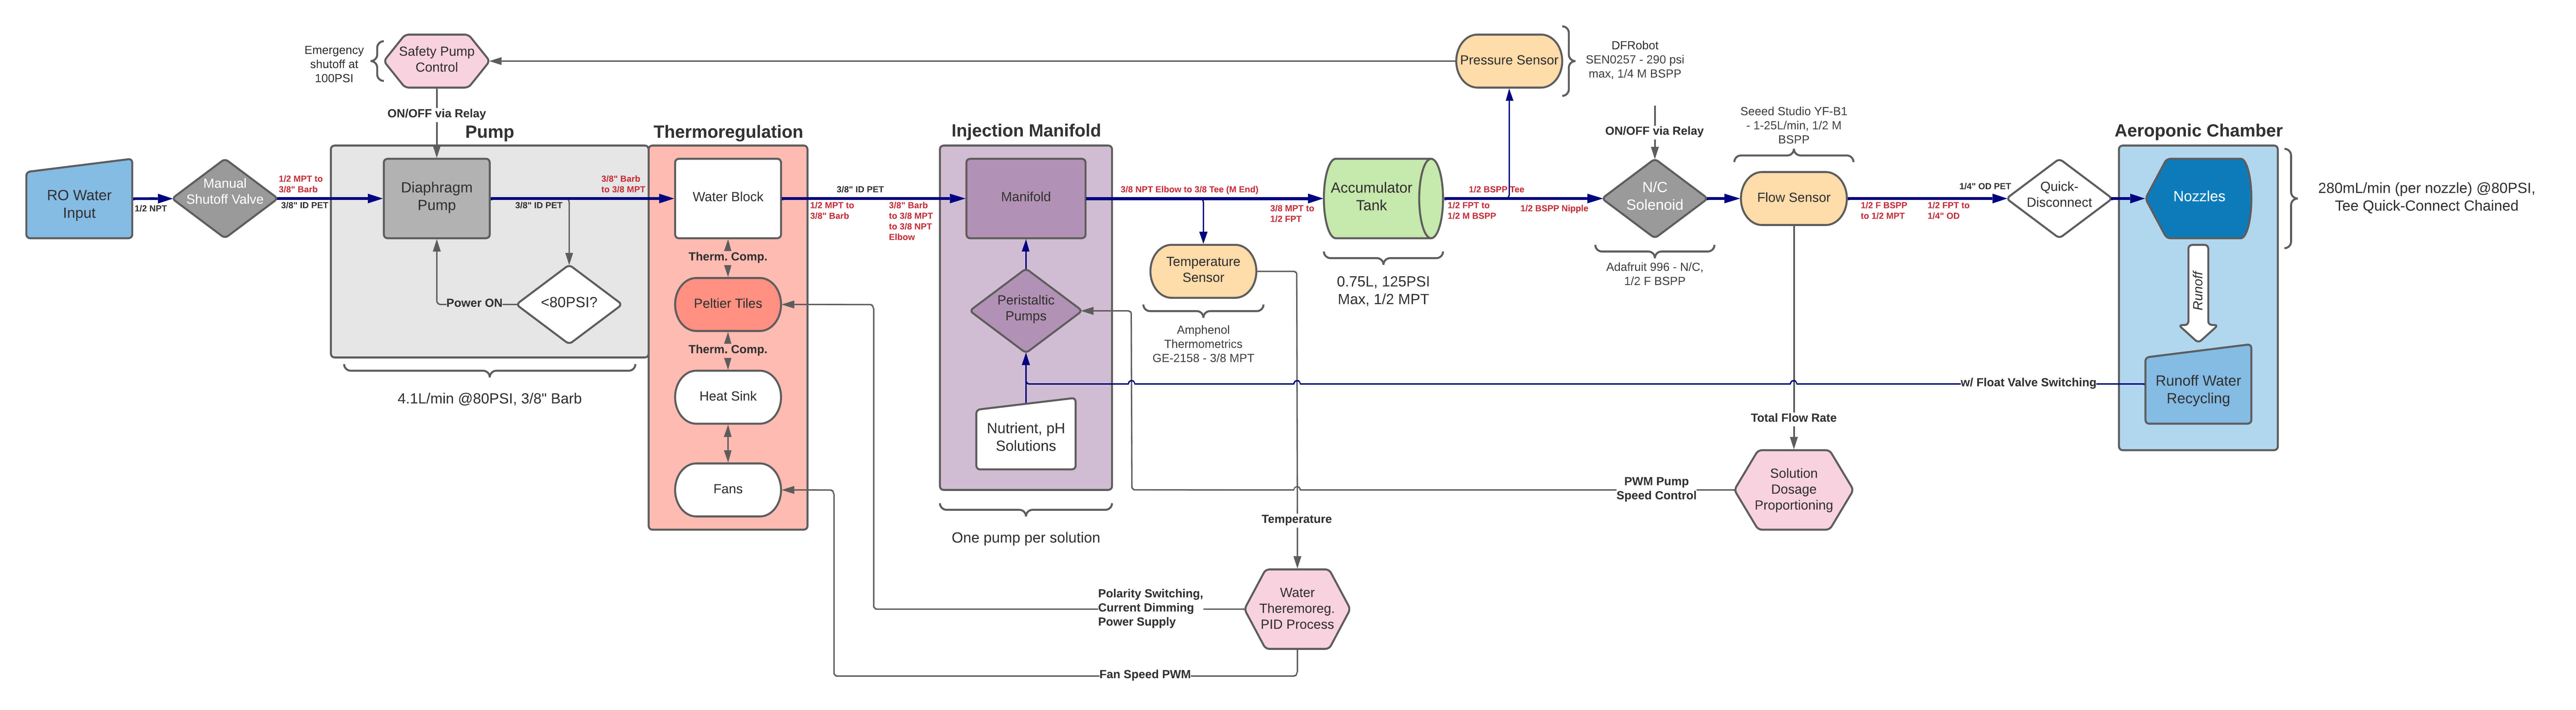
\includegraphics[width=\textwidth]{../assets/figures/aeroponics_plumbing.png}}
    \caption{Aeroponics plumbing diagram.}
    \label{fig:aeroponics_plumbing}
\end{figure}

\begin{figure}[h!]
    \centering
    \frame{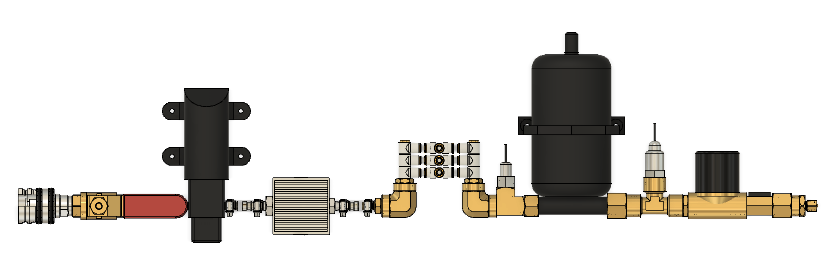
\includegraphics[width=\textwidth]{../assets/figures/aeroponics_supply.png}}
    \caption{Aeroponics supply system.}
    \label{fig:aeroponics_supply}
\end{figure}

% TODO Pump model figure

\clearpage

\clearpage

\subsection{Lighting}
\label{sec:lighting}

\textbf{Purpose}: Discrete light spectrum and intensity control to provide all light necessary for plant growth, as well as sanitization.

\textbf{Function}:
\begin{itemize}
    \item \textbf{Inputs}: Power, lighting spectrum-intensity control signal (aka per-LED modulation signals)
    \item \textbf{Outputs}: Light
\end{itemize}

\textbf{Method}:
\begin{enumerate}
    \item \textit{Setup}:
    \begin{enumerate}
        \item Connect power and spectrum-intensity control signal to driver board;
        \item Mount driver board and many LED boards to lighting tray;
        \item Daisy-chain LED boards, connect first and last to driver board;
    \end{enumerate}
    \item \textit{Testing}:
    \begin{itemize}
        \item Spectrum-intensity distribution control signal modulates LED power as expected;
        \item Passive heat sinks dissipate enough heat;
    \end{itemize}
    \item \textit{Process}:
    \begin{enumerate}
        \item Power is delivered to drivers;
        \item Control signals "dim" drivers to modulate intensity distribution across spectrum;
        \item Power drivers power LEDs (one per wavelength/"series");
        \item LEDs emit light;
    \end{enumerate}
    \item \textit{Shutdown}:
    \begin{enumerate}
        \item Disconnect power and signals;
        \item Disconnect and dismount boards;
    \end{enumerate}
\end{enumerate}

\textbf{Features}:
\begin{itemize}
    \item \textit{LED Lights}: LEDs offer high power output, better efficiency and thermal management, lower footprint, and precise wavelengths while minimizing risk of damaging plant tissues. Many discretely-controlled wavelength options/"series" enable wide and fine control of intensity-spectrum distribution, with a focus on Photosynthetically-Active Radiation (PAR), as well as sanitization wavelengths and wavelengths to induce specific phenotypic and chemical changes. Located across multiple smaller daisy-chained PCBs to minimize cost. LED series include:
    \begin{itemize}
        \item Ultraviolet (267nm\footnote{This is the ideal wavelength for targeting a variety of pathogens, notably \textit{E. coli} \cite{uvecoli}}) \cite{led_uv};
        \item Blue (448nm) \cite{led_xpg3};
        \item Cool White (5700K) \cite{led_xpg3};
        \item Warm White (2700K) \cite{led_xpg3};
        \item Red (645nm) \cite{led_xpg3};
        \item Near-Infrared (730nm) \cite{led_xpe2};
    \end{itemize}
    \item \textit{LED Power Drivers}: High-efficiency constant-current PWM-dimmable DC-DC buck converters, specialized for LEDs \cite{leddriver}. One per series, driving a set of identical LEDs. One driver per lighting tray.
    % \item \textit{Heat Sink}: Passive cooling solution for LEDs. Mounted to opposing face of PCB.
\end{itemize}

\clearpage

\textbf{Figures}

\begin{figure}[h!]
    \centering
    \begin{subfigure}{.34\textwidth}
        \centering
        \frame{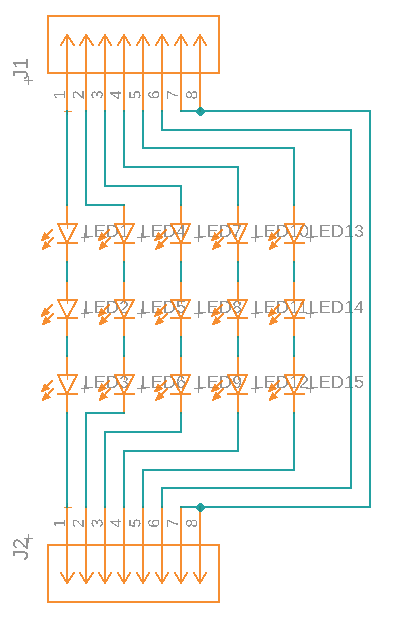
\includegraphics[width=\textwidth]{../assets/schematics/lighting_led_sch.png}}
        \caption{Schematic.}
        \label{fig:lighting_led_sch}
      \end{subfigure}
      \hspace{.08\textwidth}
      \begin{subfigure}{.35\textwidth}
        \centering
        \frame{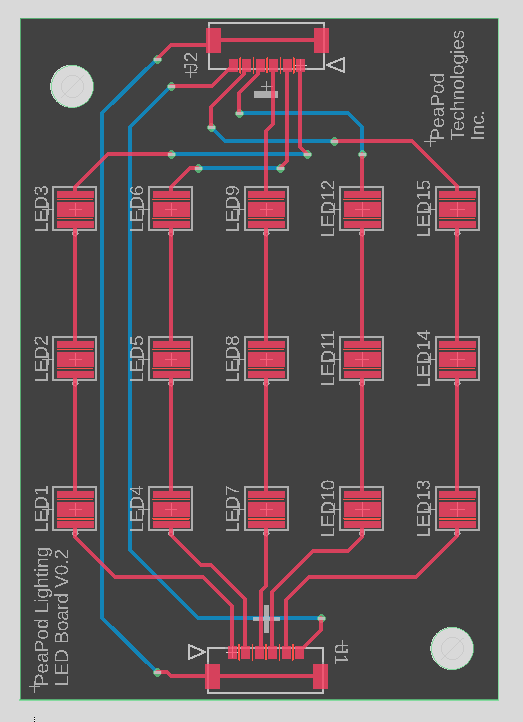
\includegraphics[width=\textwidth]{../assets/schematics/lighting_led_brd.png}}
        \caption{PCB layout.}
        \label{fig:lighting_led_brd}
      \end{subfigure}
      \caption{Lighting LED board.}
\end{figure}

\begin{figure}[h!]
    \centering
    \begin{subfigure}{.35\textwidth}
        \centering
        \frame{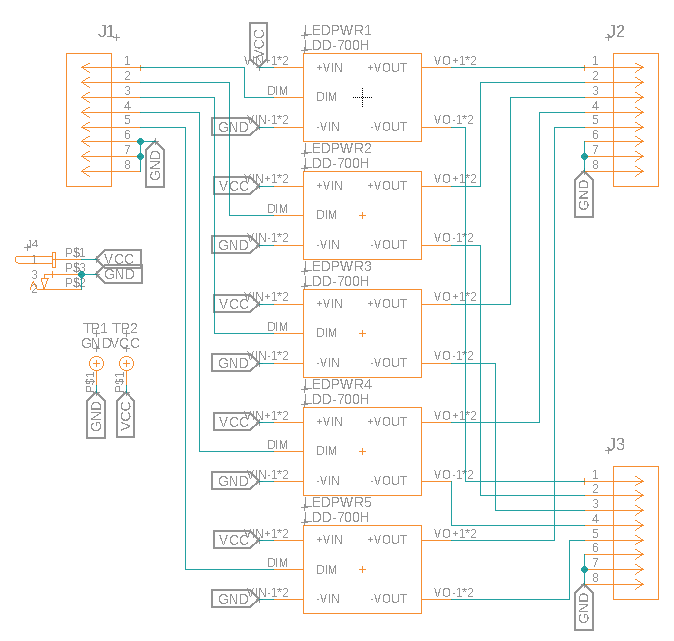
\includegraphics[width=\textwidth]{../assets/schematics/lighting_power_sch.png}}
        \caption{Schematic.}
        \label{fig:lighting_power_sch}
      \end{subfigure}
      \hspace{.02\textwidth}
      \begin{subfigure}{.6\textwidth}
        \centering
        \frame{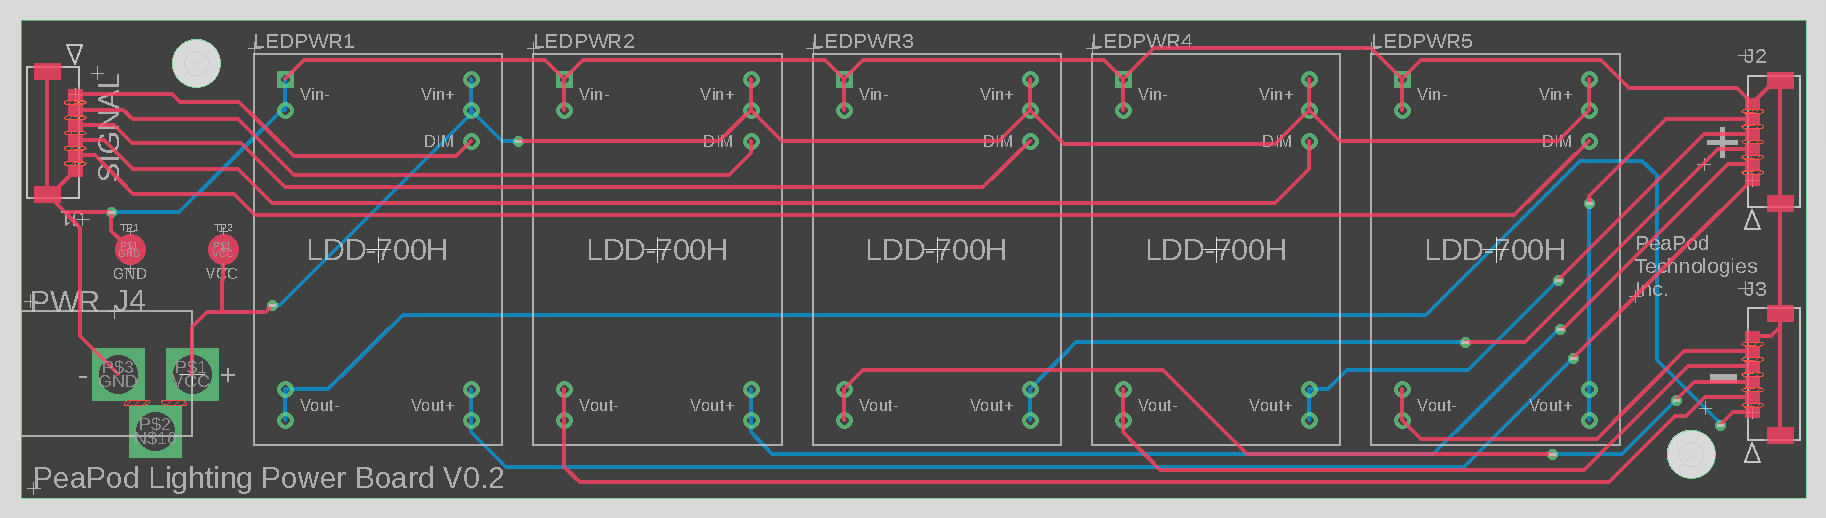
\includegraphics[width=\textwidth]{../assets/schematics/lighting_power_brd.png}}
        \caption{PCB layout.}
        \label{fig:lighting_power_brd}
      \end{subfigure}
      \caption{Lighting power board.}
\end{figure}

\clearpage

% References
\bibliographystyle{IEEEtran}
\bibliography{references}
\end{document}